%% bare_jrnl.tex
%% V1.4b
%% 2015/08/26
%% by Michael Shell
%% see http://www.michaelshell.org/
%% for current contact information.
%%
%% This is a skeleton file demonstrating the use of IEEEtran.cls
%% (requires IEEEtran.cls version 1.8b or later) with an IEEE
%% journal paper.
%%
%% Support sites:
%% http://www.michaelshell.org/tex/ieeetran/
%% http://www.ctan.org/pkg/ieeetran
%% and
%% http://www.ieee.org/

%%*************************************************************************
%% Legal Notice:
%% This code is offered as-is without any warranty either expressed or
%% implied; without even the implied warranty of MERCHANTABILITY or
%% FITNESS FOR A PARTICULAR PURPOSE! 
%% User assumes all risk.
%% In no event shall the IEEE or any contributor to this code be liable for
%% any damages or losses, including, but not limited to, incidental,
%% consequential, or any other damages, resulting from the use or misuse
%% of any information contained here.
%%
%% All comments are the opinions of their respective authors and are not
%% necessarily endorsed by the IEEE.
%%
%% This work is distributed under the LaTeX Project Public License (LPPL)
%% ( http://www.latex-project.org/ ) version 1.3, and may be freely used,
%% distributed and modified. A copy of the LPPL, version 1.3, is included
%% in the base LaTeX documentation of all distributions of LaTeX released
%% 2003/12/01 or later.
%% Retain all contribution notices and credits.
%% ** Modified files should be clearly indicated as such, including  **
%% ** renaming them and changing author support contact information. **
%%*************************************************************************


% *** Authors should verify (and, if needed, correct) their LaTeX system  ***
% *** with the testflow diagnostic prior to trusting their LaTeX platform ***
% *** with production work. The IEEE's font choices and paper sizes can   ***
% *** trigger bugs that do not appear when using other class files.       ***                          ***
% The testflow support page is at:
% http://www.michaelshell.org/tex/testflow/



\documentclass[journal]{IEEEtran}
\makeatletter
\long\def\@makecaption#1#2{\ifx\@captype\@IEEEtablestring%
\footnotesize\begin{center}{\normalfont\footnotesize #1}\\
{\normalfont\footnotesize\scshape #2}\end{center}%
\@IEEEtablecaptionsepspace
\else
\@IEEEfigurecaptionsepspace
\setbox\@tempboxa\hbox{\normalfont\footnotesize {#1.}~~ #2}%
\ifdim \wd\@tempboxa >\hsize%
\setbox\@tempboxa\hbox{\normalfont\footnotesize {#1.}~~ }%
\parbox[t]{\hsize}{\normalfont\footnotesize \noindent\unhbox\@tempboxa#2}%
\else
\hbox to\hsize{\normalfont\footnotesize\hfil\box\@tempboxa\hfil}\fi\fi}
\makeatother
%
% If IEEEtran.cls has not been installed into the LaTeX system files,
% manually specify the path to it like:
% \documentclass[journal]{../sty/IEEEtran}





% Some very useful LaTeX packages include:
% (uncomment the ones you want to load)


% *** MISC UTILITY PACKAGES ***
%
%\usepackage{ifpdf}
% Heiko Oberdiek's ifpdf.sty is very useful if you need conditional
% compilation based on whether the output is pdf or dvi.
% usage:
% \ifpdf
%   % pdf code
% \else
%   % dvi code
% \fi
% The latest version of ifpdf.sty can be obtained from:
% http://www.ctan.org/pkg/ifpdf
% Also, note that IEEEtran.cls V1.7 and later provides a builtin
% \ifCLASSINFOpdf conditional that works the same way.
% When switching from latex to pdflatex and vice-versa, the compiler may
% have to be run twice to clear warning/error messages.






% *** CITATION PACKAGES ***
%
%\usepackage{cite}
% cite.sty was written by Donald Arseneau
% V1.6 and later of IEEEtran pre-defines the format of the cite.sty package
% \cite{} output to follow that of the IEEE. Loading the cite package will
% result in citation numbers being automatically sorted and properly
% "compressed/ranged". e.g., [1], [9], [2], [7], [5], [6] without using
% cite.sty will become [1], [2], [5]--[7], [9] using cite.sty. cite.sty's
% \cite will automatically add leading space, if needed. Use cite.sty's
% noadjust option (cite.sty V3.8 and later) if you want to turn this off
% such as if a citation ever needs to be enclosed in parenthesis.
% cite.sty is already installed on most LaTeX systems. Be sure and use
% version 5.0 (2009-03-20) and later if using hyperref.sty.
% The latest version can be obtained at:
% http://www.ctan.org/pkg/cite
% The documentation is contained in the cite.sty file itself.




\usepackage[inline]{enumitem}
\usepackage[english]{babel}
% *** GRAPHICS RELATED PACKAGES ***
%
\ifCLASSINFOpdf
\usepackage[pdftex]{graphicx}
%\usepackage{caption}
  % declare the path(s) where your graphic files are
\graphicspath{{image/}}
  % and their extensions so you won't have to specify these with
  % every instance of \includegraphics
 \DeclareGraphicsExtensions{.pdf,.jpeg,.png}
\else
  % or other class option (dvipsone, dvipdf, if not using dvips). graphicx
  % will default to the driver specified in the system graphics.cfg if no
  % driver is specified.
  % \usepackage[dvips]{graphicx}
  % declare the path(s) where your graphic files are
  % \graphicspath{{../eps/}}
  % and their extensions so you won't have to specify these with
  % every instance of \includegraphics
  % \DeclareGraphicsExtensions{.eps}
 \fi
% graphicx was written by David Carlisle and Sebastian Rahtz. It is
% required if you want graphics, photos, etc. graphicx.sty is already
% installed on most LaTeX systems. The latest version and documentation
% can be obtained at: 
% http://www.ctan.org/pkg/graphicx
% Another good source of documentation is "Using Imported Graphics in
% LaTeX2e" by Keith Reckdahl which can be found at:
% http://www.ctan.org/pkg/epslatex
%
% latex, and pdflatex in dvi mode, support graphics in encapsulated
% postscript (.eps) format. pdflatex in pdf mode supports graphics
% in .pdf, .jpeg, .png and .mps (metapost) formats. Users should ensure
% that all non-photo figures use a vector format (.eps, .pdf, .mps) and
% not a bitmapped formats (.jpeg, .png). The IEEE frowns on bitmapped formats
% which can result in "jaggedy"/blurry rendering of lines and letters as
% well as large increases in file sizes.
%
% You can find documentation about the pdfTeX application at:
% http://www.tug.org/applications/pdftex





% *** MATH PACKAGES ***
%
%\usepackage{mathtools} 
\usepackage{amsmath}
\usepackage{siunitx}
\usepackage{multirow}
% A popular package from the American Mathematical Society that provides
% many useful and powerful commands for dealing with mathematics.
%
% Note that the amsmath package sets \interdisplaylinepenalty to 10000
% thus preventing page breaks from occurring within multiline equations. Use:
%\interdisplaylinepenalty=2500
% after loading amsmath to restore such page breaks as IEEEtran.cls normally
% does. amsmath.sty is already installed on most LaTeX systems. The latest
% version and documentation can be obtained at:
% http://www.ctan.org/pkg/amsmath





% *** SPECIALIZED LIST PACKAGES ***
%
\usepackage{algorithm}
%\usepackage{algorithmic}
\usepackage[noend]{algpseudocode}
\renewcommand{\algorithmicrequire}{\textbf{Input:}}  % Use Input in the format of Algorithm  
\renewcommand{\algorithmicensure}{\textbf{Output:}} % Use Output in the format of Algorithm  
% algorithmic.sty was written by Peter Williams and Rogerio Brito.
% This package provides an algorithmic environment fo describing algorithms.
% You can use the algorithmic environment in-text or within a figure
% environment to provide for a floating algorithm. Do NOT use the algorithm
% floating environment provided by algorithm.sty (by the same authors) or
% algorithm2e.sty (by Christophe Fiorio) as the IEEE does not use dedicated
% algorithm float types and packages that provide these will not provide
% correct IEEE style captions. The latest version and documentation of
% algorithmic.sty can be obtained at:
% http://www.ctan.org/pkg/algorithms
% Also of interest may be the (relatively newer and more customizable)
% algorithmicx.sty package by Szasz Janos:
% http://www.ctan.org/pkg/algorithmicx




% *** ALIGNMENT PACKAGES ***
%
%\usepackage{array}
% Frank Mittelbach's and David Carlisle's array.sty patches and improves
% the standard LaTeX2e array and tabular environments to provide better
% appearance and additional user controls. As the default LaTeX2e table
% generation code is lacking to the point of almost being broken with
% respect to the quality of the end results, all users are strongly
% advised to use an enhanced (at the very least that provided by array.sty)
% set of table tools. array.sty is already installed on most systems. The
% latest version and documentation can be obtained at:
% http://www.ctan.org/pkg/array


% IEEEtran contains the IEEEeqnarray family of commands that can be used to
% generate multiline equations as well as matrices, tables, etc., of high
% quality.




% *** SUBFIGURE PACKAGES ***
%\ifCLASSOPTIONcompsoc
%  \usepackage[caption=false,font=normalsize,labelfont=sf,textfont=sf]{subfig}
%\else
%  \usepackage[caption=false,font=footnotesize]{subfig}
%\fi
% subfig.sty, written by Steven Douglas Cochran, is the modern replacement
% for subfigure.sty, the latter of which is no longer maintained and is
% incompatible with some LaTeX packages including fixltx2e. However,
% subfig.sty requires and automatically loads Axel Sommerfeldt's caption.sty
% which will override IEEEtran.cls' handling of captions and this will result
% in non-IEEE style figure/table captions. To prevent this problem, be sure
% and invoke subfig.sty's "caption=false" package option (available since
% subfig.sty version 1.3, 2005/06/28) as this is will preserve IEEEtran.cls
% handling of captions.
% Note that the Computer Society format requires a larger sans serif font
% than the serif footnote size font used in traditional IEEE formatting
% and thus the need to invoke different subfig.sty package options depending
% on whether compsoc mode has been enabled.
%
% The latest version and documentation of subfig.sty can be obtained at:
% http://www.ctan.org/pkg/subfig




% *** FLOAT PACKAGES ***
%
\usepackage{fixltx2e}
% fixltx2e, the successor to the earlier fix2col.sty, was written by
% Frank Mittelbach and David Carlisle. This package corrects a few problems
% in the LaTeX2e kernel, the most notable of which is that in current
% LaTeX2e releases, the ordering of single and double column floats is not
% guaranteed to be preserved. Thus, an unpatched LaTeX2e can allow a
% single column figure to be placed prior to an earlier double column
% figure.
% Be aware that LaTeX2e kernels dated 2015 and later have fixltx2e.sty's
% corrections already built into the system in which case a warning will
% be issued if an attempt is made to load fixltx2e.sty as it is no longer
% needed.
% The latest version and documentation can be found at:
% http://www.ctan.org/pkg/fixltx2e


%\usepackage{stfloats}
% stfloats.sty was written by Sigitas Tolusis. This package gives LaTeX2e
% the ability to do double column floats at the bottom of the page as well
% as the top. (e.g., "\begin{figure*}[!b]" is not normally possible in
% LaTeX2e). It also provides a command:
%\fnbelowfloat
% to enable the placement of footnotes below bottom floats (the standard
% LaTeX2e kernel puts them above bottom floats). This is an invasive package
% which rewrites many portions of the LaTeX2e float routines. It may not work
% with other packages that modify the LaTeX2e float routines. The latest
% version and documentation can be obtained at:
% http://www.ctan.org/pkg/stfloats
% Do not use the stfloats baselinefloat ability as the IEEE does not allow
% \baselineskip to stretch. Authors submitting work to the IEEE should note
% that the IEEE rarely uses double column equations and that authors should try
% to avoid such use. Do not be tempted to use the cuted.sty or midfloat.sty
% packages (also by Sigitas Tolusis) as the IEEE does not format its papers in
% such ways.
% Do not attempt to use stfloats with fixltx2e as they are incompatible.
% Instead, use Morten Hogholm'a dblfloatfix which combines the features
% of both fixltx2e and stfloats:
%
% \usepackage{dblfloatfix}
% The latest version can be found at:
% http://www.ctan.org/pkg/dblfloatfix




%\ifCLASSOPTIONcaptionsoff
%  \usepackage[nomarkers]{endfloat}
% \let\MYoriglatexcaption\caption
% \renewcommand{\caption}[2][\relax]{\MYoriglatexcaption[#2]{#2}}
%\fi
% endfloat.sty was written by James Darrell McCauley, Jeff Goldberg and 
% Axel Sommerfeldt. This package may be useful when used in conjunction with 
% IEEEtran.cls'  captionsoff option. Some IEEE journals/societies require that
% submissions have lists of figures/tables at the end of the paper and that
% figures/tables without any captions are placed on a page by themselves at
% the end of the document. If needed, the draftcls IEEEtran class option or
% \CLASSINPUTbaselinestretch interface can be used to increase the line
% spacing as well. Be sure and use the nomarkers option of endfloat to
% prevent endfloat from "marking" where the figures would have been placed
% in the text. The two hack lines of code above are a slight modification of
% that suggested by in the endfloat docs (section 8.4.1) to ensure that
% the full captions always appear in the list of figures/tables - even if
% the user used the short optional argument of \caption[]{}.
% IEEE papers do not typically make use of \caption[]'s optional argument,
% so this should not be an issue. A similar trick can be used to disable
% captions of packages such as subfig.sty that lack options to turn off
% the subcaptions:
% For subfig.sty:
% \let\MYorigsubfloat\subfloat
% \renewcommand{\subfloat}[2][\relax]{\MYorigsubfloat[]{#2}}
% However, the above trick will not work if both optional arguments of
% the \subfloat command are used. Furthermore, there needs to be a
% description of each subfigure *somewhere* and endfloat does not add
% subfigure captions to its list of figures. Thus, the best approach is to
% avoid the use of subfigure captions (many IEEE journals avoid them anyway)
% and instead reference/explain all the subfigures within the main caption.
% The latest version of endfloat.sty and its documentation can obtained at:
% http://www.ctan.org/pkg/endfloat
%
% The IEEEtran \ifCLASSOPTIONcaptionsoff conditional can also be used
% later in the document, say, to conditionally put the References on a 
% page by themselves.




% *** PDF, URL AND HYPERLINK PACKAGES ***
%
%\usepackage{url}
% url.sty was written by Donald Arseneau. It provides better support for
% handling and breaking URLs. url.sty is already installed on most LaTeX
% systems. The latest version and documentation can be obtained at:
% http://www.ctan.org/pkg/url
% Basically, \url{my_url_here}.




% *** Do not adjust lengths that control margins, column widths, etc. ***
% *** Do not use packages that alter fonts (such as pslatex).         ***
% There should be no need to do such things with IEEEtran.cls V1.6 and later.
% (Unless specifically asked to do so by the journal or conference you plan
% to submit to, of course. )


% correct bad hyphenation here
\hyphenation{op-tical net-works semi-conduc-tor}


\begin{document}

%
% paper title
% Titles are generally capitalized except for words such as a, an, and, as,
% at, but, by, for, in, nor, of, on, or, the, to and up, which are usually
% not capitalized unless they are the first or last word of the title.
% Linebreaks \\ can be used within to get better formatting as desired.
% Do not put math or special symbols in the title.
\title{Human Activity Detection and Coarse-Localization Outdoors Using Micro-Doppler Signatures}
%
%
% author names and IEEE memberships
% note positions of commas and nonbreaking spaces ( ~ ) LaTeX will not break
% a structure at a ~ so this keeps an author's name from being broken across
% two lines.
% use \thanks{} to gain access to the first footnote area
% a separate \thanks must be used for each paragraph as LaTeX2e's \thanks
% was not built to handle multiple paragraphs
%

\author{Fei~Luo,
		Stefan~Posland,
        and~Eliane~Bodanese% <-this % stops a space
\thanks{Manuscript revised September 22, 2018.}
\thanks{F. Luo is with the School of Electronic Engineering and Computer Science, Queen Mary University of London, London, UK, E1 4NS  e-mail: f.luo@qmul.ac.uk.}% <-this % stops a space
\thanks{The author sequence of this paper follows the “first-last-author-emphasis” norm (FLAE).}}

% note the % following the last \IEEEmembership and also \thanks - 
% these prevent an unwanted space from occurring between the last author name
% and the end of the author line. i.e., if you had this:
% 
% \author{....lastname \thanks{...} \thanks{...} }
%                     ^------------^------------^----Do not want these spaces!
%
% a space would be appended to the last name and could cause every name on that
% line to be shifted left slightly. This is one of those "LaTeX things". For
% instance, "\textbf{A} \textbf{B}" will typeset as "A B" not "AB". To get
% "AB" then you have to do: "\textbf{A}\textbf{B}"
% \thanks is no different in this regard, so shield the last } of each \thanks
% that ends a line with a % and do not let a space in before the next \thanks.
% Spaces after \IEEEmembership other than the last one are OK (and needed) as
% you are supposed to have spaces between the names. For what it is worth,
% this is a minor point as most people would not even notice if the said evil
% space somehow managed to creep in.



% The paper headers
\markboth{Journal of IEEE Transactions on Geoscience and Remote Sensing,~Vol.~14, No.~23, September~2018}%
{Shell \MakeLowercase{\textit{et al.}}: Human Activity Detection and Coarse-Localization Outdoors Using Micro-Doppler Signatures}
% The only time the second header will appear is for the odd numbered pages
% after the title page when using the twoside option.
% 
% *** Note that you probably will NOT want to include the author's ***
% *** name in the headers of peer review papers.                   ***
% You can use \ifCLASSOPTIONpeerreview for conditional compilation here if
% you desire.




% If you want to put a publisher's ID mark on the page you can do it like
% this:
%\IEEEpubid{0000--0000/00\$00.00~\copyright~2015 IEEE}
% Remember, if you use this you must call \IEEEpubidadjcol in the second
% column for its text to clear the IEEEpubid mark.



% use for special paper notices
%\IEEEspecialpapernotice{(Invited Paper)}




% make the title area
\maketitle

% As a general rule, do not put math, special symbols or citations
% in the abstract or keywords.
\begin{abstract}
Human activity detection in outdoor environments is emerging as a very important research field due to its potential application in surveillance, assisted living, search and rescue, and military. On such applications, it is important to have a detailed information about the target, for example, if the detected target is a single person or a group of people, what activity the target is performing, and the rough location of the target. In this paper, we propose novel usage approaches of machine learning techniques to perform human recognition, human activity detection, people counting, and coarse-grained localization by classifying micro-Doppler signatures obtained from a low-cost and low-power radar system. Along with the use of a low-cost, low-power radar system, the experiments presented and evaluated in this paper were performed outdoors with a high-level of clutter, providing important findings that were not previously investigated in the literature on these same conditions. For the feature extraction of the micro-Doppler signatures, a two-directional two-dimensional principal component analysis (2D2PCA) was applied. The results show that the use of this technique greatly improved the classification rate of the Support Vector Machine (SVM) and the \textit{k}-nearest neighbor (\textit{k}NN) classifiers. In addition, we designed and implemented a Convolutional Neural Network (CNN) for the target classifications of type, number, activity, and coarse localization. The classification results obtained by using our CNN model were superior to the ones obtained using the SVM and the \textit{k}NN. This paper also investigates the frame length of the sliding window, the angle of the direction of movement, and the number of radars used in the experiment set up, providing valuable guidelines for machine learning modeling and experimental setup of micro-Doppler based research and applications.
\end{abstract}

% Note that keywords are not normally used for peerreview papers.
\begin{IEEEkeywords}
Micro-Doppler, Machine Learning Techniques, CNN, human activity detection, coarse-grained localization, people counting.
\end{IEEEkeywords}






% For peer review papers, you can put extra information on the cover
% page as needed:
% \ifCLASSOPTIONpeerreview
% \begin{center} \bfseries EDICS Category: 3-BBND \end{center}
% \fi
%
% For peerreview papers, this IEEEtran command inserts a page break and
% creates the second title. It will be ignored for other modes.
\IEEEpeerreviewmaketitle



\section{Introduction}
% The very first letter is a 2 line initial drop letter followed
% by the rest of the first word in caps.
% 
% form to use if the first word consists of a single letter:
% \IEEEPARstart{A}{demo} file is ....
% 
% form to use if you need the single drop letter followed by
% normal text (unknown if ever used by the IEEE):
% \IEEEPARstart{A}{}demo file is ....
% 
% Some journals put the first two words in caps:
% \IEEEPARstart{T}{his demo} file is ....
% 
% Here we have the typical use of a "T" for an initial drop letter
% and "HIS" in caps to complete the first word.

% You must have at least 2 lines in the paragraph with the drop letter
% (should never be an issue)
\IEEEPARstart{T}{he} detection, recognition, and classification of human targets and human activities are an increasingly important topic in many applications, such as surveillance, search and rescue, and patient/elderly monitoring. Numerous sensors, such as cameras, LIDAR \cite{madevice2018} and radars, are employed to achieve contactless measurement of humans and human kinetic characteristics. Although a wide variety of sensors exist, Doppler radar is emerging as an increasingly popular device that it is especially useful for motion analysis \cite{narayanan2015radar}. Unlike other sensor technologies, it is all-weather, it works day-and-night, and operates in non-line of sight situations such as through building walls, clothes, and foliage \cite{ram2008simulation}. It is non-intrusive, and it does not generate privacy concerns because the identity or personal identifiable features of a target cannot be obtained with radar detection. Furthermore, low-cost and low-power radar components are becoming more available, which makes Doppler radars more suitable to be deployed outdoors and on a larger scale.

Human activity recognition and classification can be obtained by comparing the differences in the radar micro-Doppler signatures of different targets and activities. A moving target relative to a radar sensor induces a frequency shift of the echo as a result of the well-known Doppler Effect. Additional movements of smaller parts of the target, called micro-motions, will result in additional modulation of the main Doppler frequency shift, known as the \textit{\textbf{micro-Doppler effect}} \cite{balleri2011classification,dura2011human}. The distinctive characteristics of the observed micro-Doppler effect of an object or a process are called \textit{\textbf{micro-Doppler signatures}} \cite{chen2014micro}. For a human activity, a unique micro-Doppler signature is the periodic motion of arms and legs that produce sidebands to the main Doppler frequency \cite{tivive2013image}. Micro-Doppler signatures are typically represented using joint time-frequency analysis such as short-time Fourier transform (STFT) \cite{tivive2013image,chen2000time}.

  In recent years, there has been a great research interest in human activity classification using micro-Doppler signatures \cite{narayanan2015radar,tivive2013image,garcia2014analysis,kim2015human}. In \cite{ccaugliyan2015micro}, a low-power pulse-Doppler radar that operates at 5.8 GHz was used to collect the micro-Doppler signatures of three different activities (walking, running, and crawling) performed by four subjects on a treadmill. Kim and Lin \cite{kim2009human} used a 2.4-GHz Doppler radar to classify seven human activities, including, for example, running, walking, and boxing. I. Bilik et al. \cite{bilik2006gmm} employed a Pulse-Doppler radar operating at 9 GHz to perform automatic target recognition on multiple people, wheeled vehicles, tracked vehicles, and animals. D. P. Fairchild et al.\cite{fairchild2016multistatic} built a bistatic radar system operating at 4 GHz to differentiate three human motions, such as no activity, arm swinging, and picking up an object.
 
In the published works above, various methods, such as Principle Component Analysis (PCA) \cite{mobasseri2009time}, Empirical Mode Decomposition (EMD) \cite{fairchild2014classification}, and Singular Value Decomposition (SVD) \cite{fioranelli2015classification,fioranelli2016performance} were used to extract the micro-Doppler features. These are computer algorithms that extract features automatically and they are more efficient and informative when compared to handcrafted feature extraction, where features are extracted manually by human visual judgement like in \cite{ccaugliyan2015micro,kim2009human,zenaldin2016radar,bjorklund2011millimeter}. 

After being extracted, the micro-Doppler features are fed into classifiers. The most used classifiers in micro-Doppler based human activity detection are Support Vector Machine (SVM) \cite{kim2009human,zenaldin2016radar,zabalza2014robust}, \textit{k}-Nearest-Neighbour (\textit{k}NN) \cite{ccaugliyan2015micro} and Na\"ive Bayes \cite{nanzer2009bayesian}. Deep neural networks have been used to classify micro-Doppler signatures only recently. For example, the authors of \cite{kim2016human} proposed the use of Deep Convolutional Neural Networks (DCNNs) for human detection and activity classification; in \cite{kim2016classification} the authors used DCNNs to classify human swimming styles; and in \cite{tahmoush2010ugs} a DCNN outperformed SVM and \textit{k}NN by a wide margin when classifying multi-target human gait. However, this previous work was implemented indoors or in environments with low levels of clutter. It is more challenging to perform human activity detection outdoors. The complex terrain, the trees, and incident foliage create spatial clutter and introduce noise that results in lower signal-to-noise ratio (SNR). Additionally, animals may be confused with humans, creating false positives. Hence, before performing human activity detection, it is also important to differentiate humans from confusers. Micro-Doppler signatures from animal and vehicle confusers have been investigated, for example in \cite{miller2013micro,lee2017classification,smith2008naive}.

Some research work on human activity recognition outdoors using micro-Doppler signature has considered clutter and noise \cite{zenaldin2016radar,tahmoush2010ugs,karabacak2015knowledge,tahmoush2009radar}. However, the radars used in those works are high--power radars and need constant mains power to function, which is an important shortcoming for lasting continuous detection in outdoors, especially in areas where the electricity supply may be scarce or absent. Our proposed research addresses this problem by using low-power pulsed Doppler radars operating at 5.8 GHz that allows long-lasting battery powered operation. This is an important factor for outdoor operations of surveillance or monitoring.

The outdoors usually comprises a large area, and it is important not only to know what the target is doing but also where the target is.  It is not feasible to perform localization by using range-Doppler analysis in this research, because the pulsed Doppler radar implemented here cannot provide the information of the azimuth and the distance to the target. To the best of our knowledge, there is no relevant literature research applying micro-Doppler signature classification for coarse-grained location estimation. However, our research is investigating ways to estimate approximately the distance between the radar and the target according to the changing intensity of the micro-Doppler signatures due to the atmospheric attenuation, and reflections of the target and the environment. In this research, the radar detection range is split into three non-overlapping ranges, the micro-Doppler signatures are labeled with the correspondent range. Machine learning algorithms such as SVM, \textit{k}NN, and DCNNs are implemented to classify the micro-Doppler signatures based on those ranges.

The main contributions of this paper can be summarized as follows:
\begin{enumerate}
\item The research presented in this paper uses low-cost and low-power Doppler radars to perform micro-Doppler signature based human activity detection in outdoor environments (complex terrains cluttered with plants and animals). This study provides new approaches of usage and results for low-cost radars that have not previously been investigated in the literature.
\item The experiments presented in this paper not only classify human activity but can also differentiate between humans and animals and can count people. For the activity classification, two types of human activities were investigated (walking and running). The differentiation between humans and animals is used to reduce the rate of false alarms resulting from animals. People counting provides the number of individuals performing an activity that could be valuable information in applications pertaining to surveillance, monitoring.
\item An image feature extraction method-2D2PCA has been applied to extract the micro-Doppler features. This paper shows that the use of 2D2PCA improves the performance of SVM and \textit{k}NN greatly. Although CNN can extract features automatically and achieves the best performance, the training process is long and the computation is more costly. By combining 2D2PCA and SVM one can achieve results close to those using CNN, but in less time and with a lower computation cost. The results presented in this paper shows that applying SVM+2D2PCA may provide a more cost-effective and time-efficient option if the application can absorb a small compromise in the performance of the micro-Doppler signature classification.
\item This research investigates a way to roughly estimate the location of human activity by applying micro-Doppler signature classification for coarse-grained location estimation -- this is novel.
\item This research also investigates the effects of frame length of the sliding window, angles of the movement, and the number of radars on the classification performance. Thus it provides valuable guidelines for machine learning modelling optimization and experiment setup for micro-Doppler based research and applications.
\end{enumerate}

The remainder of this paper is organized as follows. Section II introduces the fundamental concepts of micro-Doppler, the characteristics of the Bumblebee radar, and describes the composition of the Doppler radar system in detail. Section III describes the three experiments performed in this research; it presents and analyzes the pattern of spectrograms that were generated by the different subjects, angles, and ranges. Section IV shows how the radar signals were collected and stored in a database, the methods used for data processing and the composition of the samples after data processing. Section V describes the mathematical fundamentals of 2D2PCA and how it can be applied to micro-Doppler feature extraction. Section VI presents the concepts of CNNs and our proposed structure of the CNN for classification of the gathered Micro-Doppler signatures, and models the SVM and \textit{k}NN classifiers by optimizing and listing their hyper-parameters. Section VII presents, analyzes, and compares the classification results of the five classifiers for each of the desired detections (human activity, people counting, human versus animal confuser, and coarse localization). Section VIII investigates the effects of the frame length of the sliding window, angles of the movement, and the number of radars. Section IX summarizes the contributions and discusses the future prospects of the research.

\section{Radar micro-Doppler}
\subsection{Micro-Doppler}
The concept of micro-Doppler was first proposed by Chen in 2000 \cite{tahmoush2009remote}. Micro-Doppler signatures reflect the periodic kinetic characteristics of a moving object. Modulations of the radar resulted from the arms, the legs and even the body sway have been investigated by researchers \cite{ram2008simulation,tahmoush2009radar,zhang2007acoustic}. 

Given an electromagnetic wave transmitted by an RF radar, the frequency of the received signals due to a moving target with a constant radial velocity $v$ with respect to the radar is:
\begin{equation}
f=f_0 (1+2v/c),
\end{equation}
where $f_0$ is the carrier frequency of the radar and  $c$ is the speed of the light. The Doppler frequency shift due to the target is:
\begin{equation}
f_D=f_0  (2v/c),
\end{equation}
which is proportional to the velocity of the target relative to the radar.

In the case of an articulated body such as a walking person, the torso, each arm and each leg has its own velocity, and even when the torso's velocity is constant, the velocity of the limbs changes over time \cite{zhang2007acoustic}. The Doppler signature $f_{Dsig}$ for such a complex object has multiple time-dependent frequency shifted components and it is defined as:
\begin{equation}
f_{Dsig} (t)=f_0\sum_{i=1}^{N}2v_i (t)/c,
\end{equation}
where $N$ is the number of parts of the moving target, $v_i (t)$ is the velocity of each part as a function of the time. The analytic signal of the returned echo from such a target is given by: 
\begin{equation}
\hat{S}_R (t)=e^{j2 \pi f_0 t} e^{j2\pi f_{Dsig} (t)t},
\end{equation}
The combination of the received signal $\hat{S}_R (t)$ with the transmitted signal $\hat{S}_T (t)$ as follows:
\begin{equation}
\hat{S}_R (t) 〖\hat{S}_T ̂(t)〗^*=e^{j2\pi f_0 t},
\end{equation}
allows the extraction of the Doppler signature from the data. This is the component of the signal that contains the micro-Doppler information of the target and it can be used for target or activity recognition and classification. The bandwidth of the resulting signal is normally much smaller than the carrier frequency,  because the micro-Doppler information relies on the lower frequencies \cite{balleri2011classification}. The micro-Doppler signature can be represented in a two-dimensional time-frequency space using a Short Time Fourier Transform (STFT):  
\begin{equation}
\begin{split}
STFT(i,K)=&\sum_{n=0}^{N-1} x_i (n) e^{-j2\pi(nK/N) },\\& K=0,\ldots ,N-1
\end{split}
\end{equation}
where $x_i (n)$ is the sliding window with a given length $N$. The $i$th window is defined as:
\begin{equation}
x_i (n)=\hat{S}_R (n+i(N/2))w(n),
\end{equation}
where $w(n)$ is a weighting function.

The frequency resolution can be approximated as the inverse of the duration of the window:
\begin{equation}
T_w=N/f_s,
\end{equation}
where $f_s$ is the sampling rate, and therefore only Doppler shifts that are greater than $1/T_w$, corresponding to velocities
\begin{equation}\label{eq:ddf}
v>c/〖2f_o T〗_w,
\end{equation}
will be clearly visible \cite{balleri2011classification}. From Eq. (\ref{eq:ddf}), it can be shown that radars that work in higher frequencies have the additional advantage to induce a wider micro-Doppler bandwidth where small movements are more easily detected for a given frequency resolution, because the carrier frequency is higher \cite{balleri2011classification}.

In this paper, an STFT has been used to generate time-frequency spectrograms. Fig. \ref{fig_tf0} shows a spectrogram of the radar signals of a human walking indoors that were collected in this research. The spectrogram shows the evident periodic characteristics of a human activity. The fluctuations resulted by the limbs are attached to the main Doppler frequency resulted by the torso. 
\begin{figure}[!t]
\centering
%\captionsetup{justification=centering}
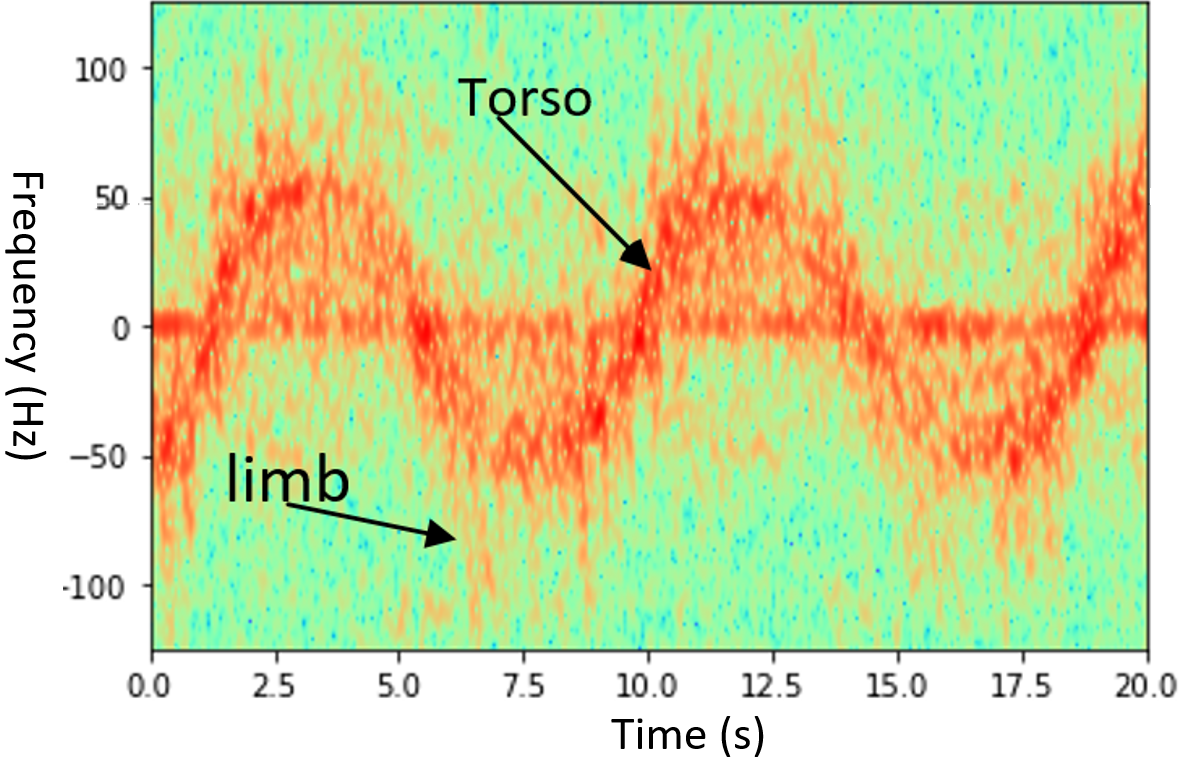
\includegraphics[width=3in]{time_frequency}
\centering
\caption{A time-frequency spectrogram of indoor human walking}
\label{fig_tf0}
\end{figure}

\subsection{The Low-power Radar System}
The Doppler radar system built in this research consists of two BumbleBee radars from Samraksh \cite{bumblebee}. The Bumblebee radar is a low-power Pulsed Doppler Radar that is designed for a variety of Wireless Sensor Network (WSN) applications. Its center frequency is 5.8 GHz; and its detection range is up to 8 meters outdoors. Unlike traditional radars, the BumbleBee is designed to be compatible at a system level with small, battery powered nodes. It only consumes about 12 mA, so when using typical 1.5v AA alkaline batteries with a capacity of 2400 mA, it can run at 100\% duty cycle for about 8 days. Each BumbleBee radar outputs data on two channels providing the in-phase  ($I$) and quadrature-phase ($Q$) signal components, which are used to form the complex signal $C=I+jQ$. The $I/Q$ output data of the BumbleBee radar represents the peak of the matched filtered data acquired for each pulse. Thus, the time interval between each data packet corresponds to the pulse repetition interval (PRI) of the radar.

Each BumbleBee radar was connected to one TelosB mote \cite{polastre2005telos} and another TelosB mote was used as a base station connected to a PC (see Fig. \ref{fig_radar}). The TelosB mote provides radio communication at low-power consumption (IEEE 802.15.4).  It has a long battery life and it is able to wake up fast from a sleep state. It is fully compatible with the open-source TinyOS, an operating system that supports large-scale, self-assembling sensor networks.
\begin{figure}[!t]
\centering
%\captionsetup{justification=centering}
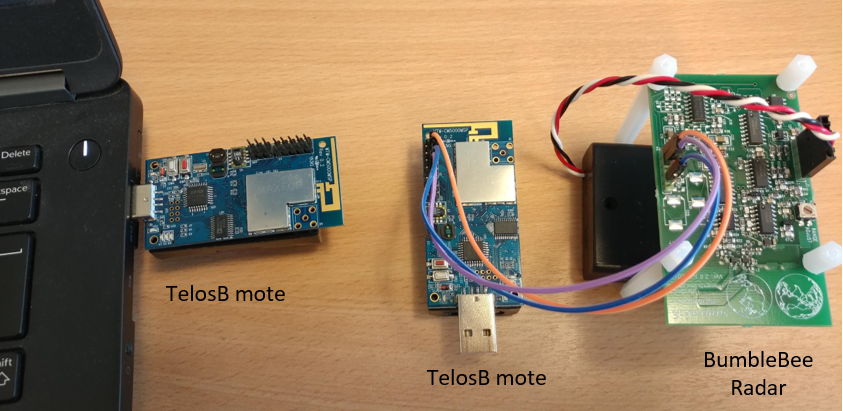
\includegraphics[width=3in]{radar}
\centering
\caption{BumbleBee radar and TelosB mote}
\label{fig_radar}
\end{figure}

In our investigation, a multi-radar system composed of two radars was used. The reason for that is because a multi-radar system collects signals of human activity from multiple angles, this provides more information for the classifiers. However, it also means more data is required to be transferred concurrently, consequently packet loss in data transmission increases in detriment to the gains in information gathering. We found that for a system set up with one base station and two radars there was an increased gain in information gathering without loss in data transmission, but for a higher number of radars the transmission data loss was noticeable.

For validating the setup of our BumbleBee radars, a corner reflector was used as a target. The corner reflector was tied to a string and hanged from the ceiling of a laboratory and pushed slightly to swing back and forth.  Our experiment followed the same set up as the corner reflector experiment presented in \cite{cagliyan2014human} that also used BumbleBee radars. The corner reflector`’s swinging was measured by the Bumblebee radars, and the collected signals were used to generate a frequency spectrogram to show the fluctuations of the reflected micro-Doppler signals. Fig. \ref{fig_validation}(a) presents the frequency spectrogram shown in \cite{cagliyan2014human} and Fig. \ref{fig_validation}(b) shows the spectrogram obtained from our radars. Both spectrograms show similar periodical fluctuations caused by the swinging of the corner reflector. In both, when the range of the swing angle declines, the amplitude of fluctuations decreases. Therefore, the setup of our Bumblebee radars was successfully validated.
\begin{figure}[!t]
\centering
%\captionsetup{justification=centering}
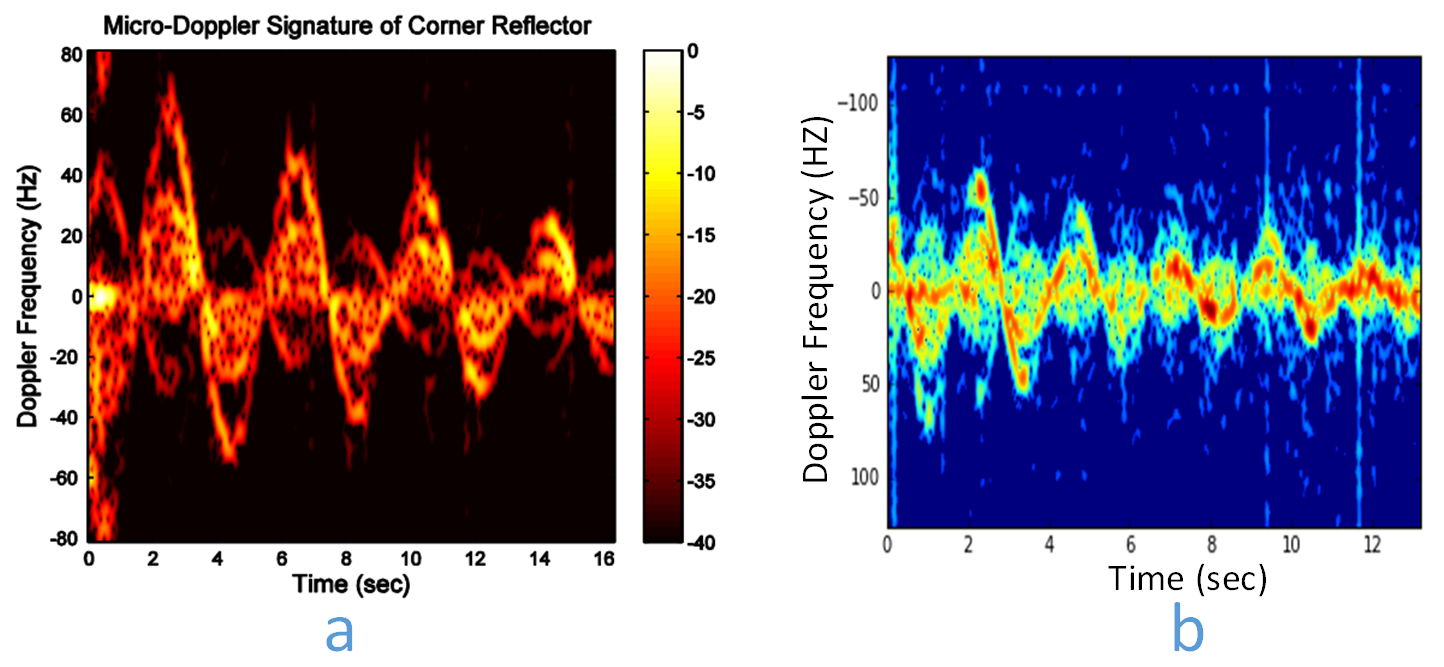
\includegraphics[width=3.5in]{validation}
\centering
\caption{Micro-Doppler signatures of a swinging corner reflector}
\label{fig_validation}
\end{figure}

The Doppler radar system was implemented outdoors. As shown in Fig.  \ref{fig_rs}, two radars (BumbleBee 1, BumbleBee 2) were placed in a straight line, eight meters apart and opposite to each other. One radar was called the \textit{primary node} (BumbleBee 1), the other was called the \textit{secondary node} (BumbleBee 2). There was a \textit{base station} (Telosb 03) connected to a laptop. The base station received data from the two Telosb motes (Telosb 01 and Telosb 02). Each mote was connected to one BumbleBee radar. The light red and light blue shadowed areas were the detection ranges of BumbleBee 1 and BumbleBee 2 respectively. The cross width of the detection ranges was from 10m to 12m. Only targets inside the detection ranges could be observed. It can be noticed that the union of two radars’ detection ranges was split into three non-overlapping ranges, which were 1-3m, 3-5m, and 5-7m relative to the primary node. The experiments were made in these three different ranges in order to tag the range labels to the micro-Doppler signatures, which were used for coarse-grained localization. The arrows represent the target movement direction relative to the radar beam. In order to investigate the effects of the angle between the direction of movement and the radar, three different directions (\ang{0}, \ang{45}, and \ang{90}) were considered. The direction of the target movements at \ang{45} was the same as at \ang{90}, however the radar beams of the primary and secondary nodes were changed to \ang{45} when performing the experiments for the \ang{45} angle.
\begin{figure}[!t]
\centering
%\captionsetup{justification=centering}
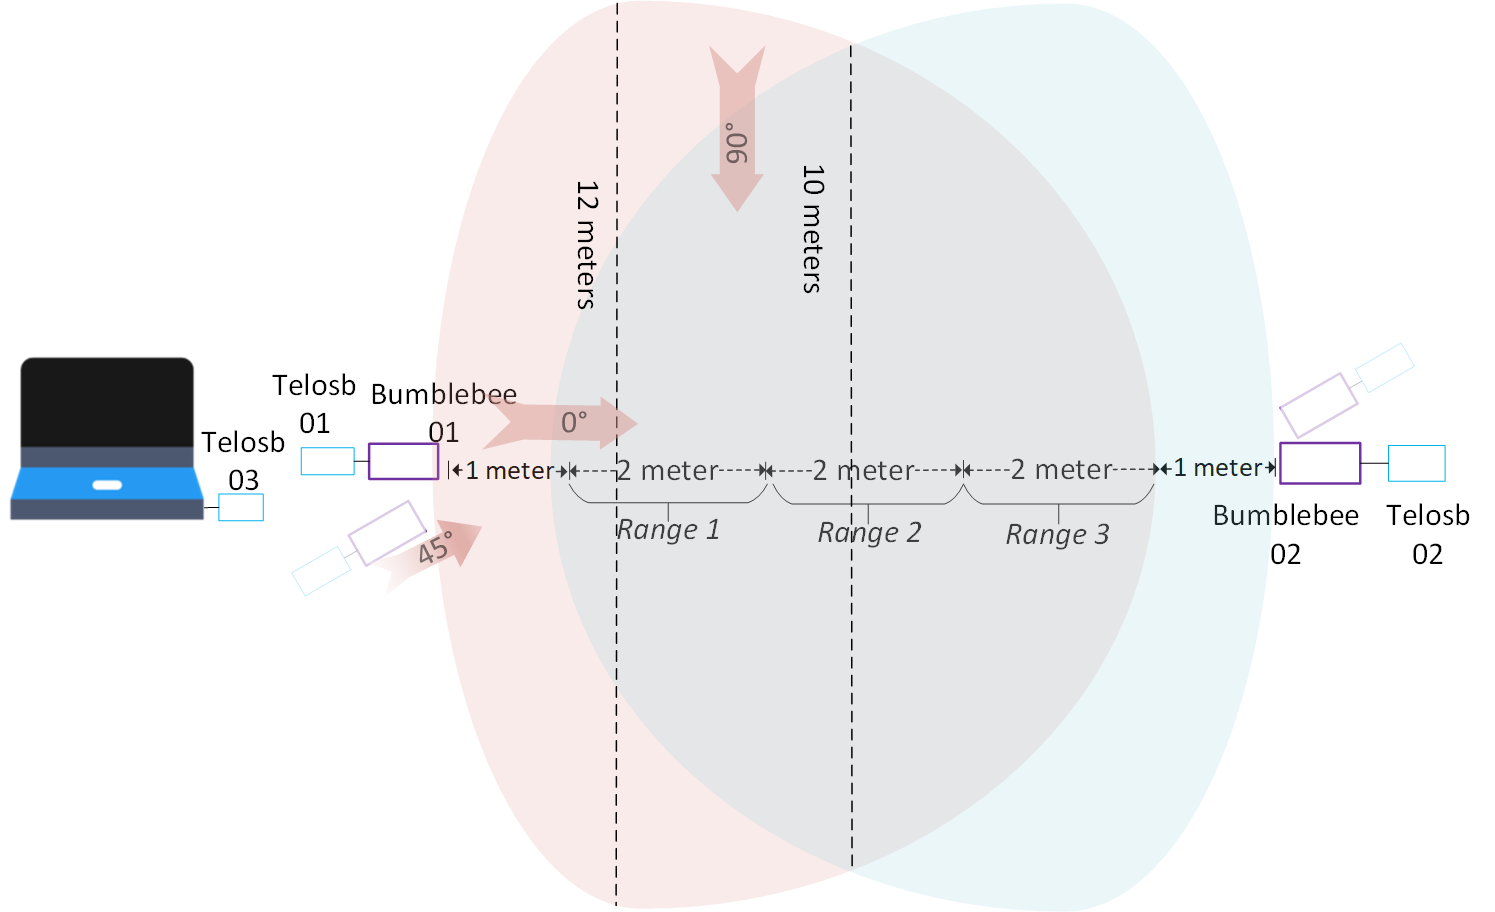
\includegraphics[width=3.6in]{radar_system}
\caption{Doppler radar system implemented in outdoors}
\label{fig_rs}
\end{figure}

\section{Experiments}
In order to investigate the effectiveness of the human activity detection outdoors using our system, four different tasks were processed in the experiments. They were human recognition, human activity classification, people counting, and coarse-grained localization. As illustrated in Fig. \ref{fig_dia}, the output metric for human recognition is whether the target is human or animal, or there is no target. If the target is human, then the system further estimates whether the target is running or walking, how many people the target represents, and the rough range that the target is located in. Although the maximum number of people counted in a group is 4 and the ranges for rough localization are relatively narrow (only 2 meters apart because of the short detection range of the Bumblebee radar), it is foreseen that the methods used here could also be applied to a greater number of people and to radars that have greater detection ranges.

Three different experiments were performed in three different outdoor locations respectively. The experimental locations were populated with trees and shrubs; they were realistic wild areas. These experiments are described in detail below:  
\begin{figure}[!t]
\centering
%\captionsetup{justification=centering}
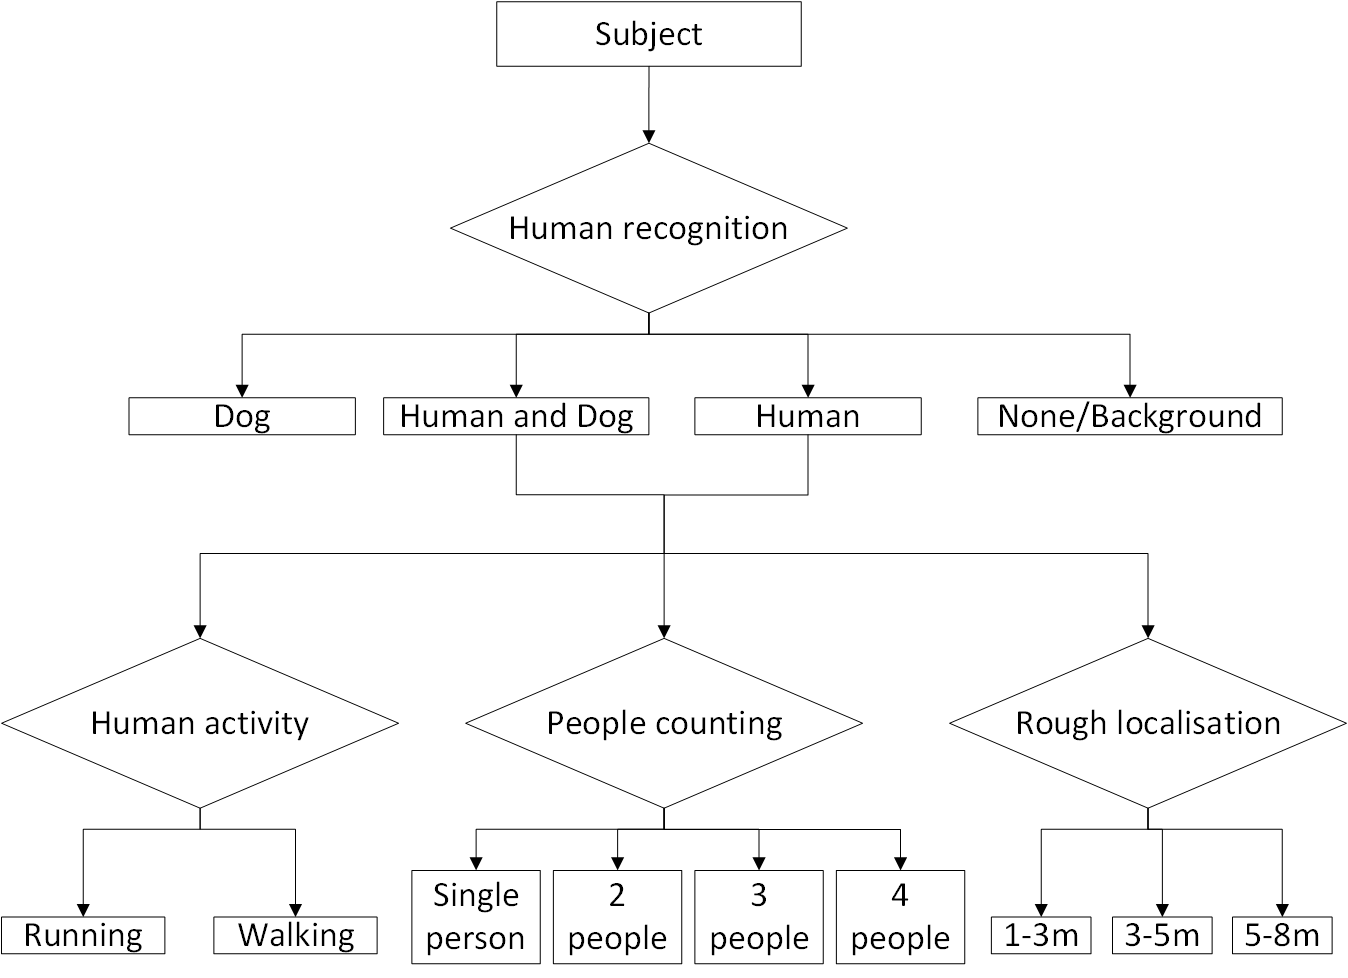
\includegraphics[width=3.5in]{diagram}
\caption{Workflow of four tasks, including human recognition, human activity \qquad detection, people counting, and coarse-grained localization}
\label{fig_dia}
\end{figure}

\textit{Case 1: Activity classification of a single person}: In this experiment, three individuals participated. Two types of activities (walking and running) were performed from three different angles ($\ang{0}$, $\ang{45}$, $\ang{90}$) relative to the radar beam. The same set of experiments was performed by each participant one at a time. At \ang{45} and \ang{90}, activities were performed in three different ranges, which were 1-3m, 3-5m, and 5-7m relative to the primary node. 

Fig. \ref{fig_mss} illustrates the micro-Doppler signatures of an individual participant walking at \ang{0}, \ang{45} and \ang{90}, which was collected by the radar system. The spectrograms were generated by a STFT with a sliding window size of 20s. As it can be seen, the spectrograms collected from outdoors are a little less clear than the ones collected indoors (as shown in Fig. 1). This is due to the complexity of the outdoor environment and a higher presence of noise. Comparing Fig. \ref{fig_mss}(a) and Fig. \ref{fig_mss}(b), the motion cycle of running is shorter than walking. There are more than three cycles in the spectrogram for running, but only 2 cycles in the spectrogram for walking. This confirms the physical fact that running takes less time to finish a motion cycle than walking. Another interesting finding is that the wave directions of Fig. \ref{fig_mss}(a) and Fig. \ref{fig_mss}(b) are opposite to the wave directions of Fig. \ref{fig_mss}(e) and Fig. \ref{fig_mss}(f), while the wave directions of Fig. \ref{fig_mss}(c) and Fig. \ref{fig_mss}(d) are the same as the Fig. \ref{fig_mss}(g) and Fig. \ref{fig_mss}(h). This is because the directions of the primary node and the secondary node are opposite to each other. When a person moves at \ang{0}, he/she is moving towards a radar and moving away from the other radar. The frequencies of the echoed wave signals of the two radars fluctuate in opposite directions. When a person moves at \ang{90} and \ang{45}, he/she gets close to or further away from both primary and second radars almost at the same time. The frequencies of the echoed wave signals of the two radars fluctuate in the same direction. Fig. \ref{fig_mss}(d) and Fig. \ref{fig_mss}(h) present more faded cycle segments, but in different positions. This is because when the participant is walking at \ang{45}, he/she is not within the detection range or he/she is at the edge of the range of each radar for a small period of time. In the spectrograms, the change in color intensity results from the changes in the radar cross-sections (RCS). The radar cross section (RCS) is the measure of a target's ability to reflect the radar signals in the direction of the radar's receiver, i.e. it is a measure of the ratio between the backscatter density in the direction of the radar (from the target) and the power density that is intercepted by the target. Larger RCS indicates a greater energy is reflected by the target, and it produces more intensive color in the spectrograms.
\begin{figure}[!t]
\centering
%\captionsetup{justification=centering}
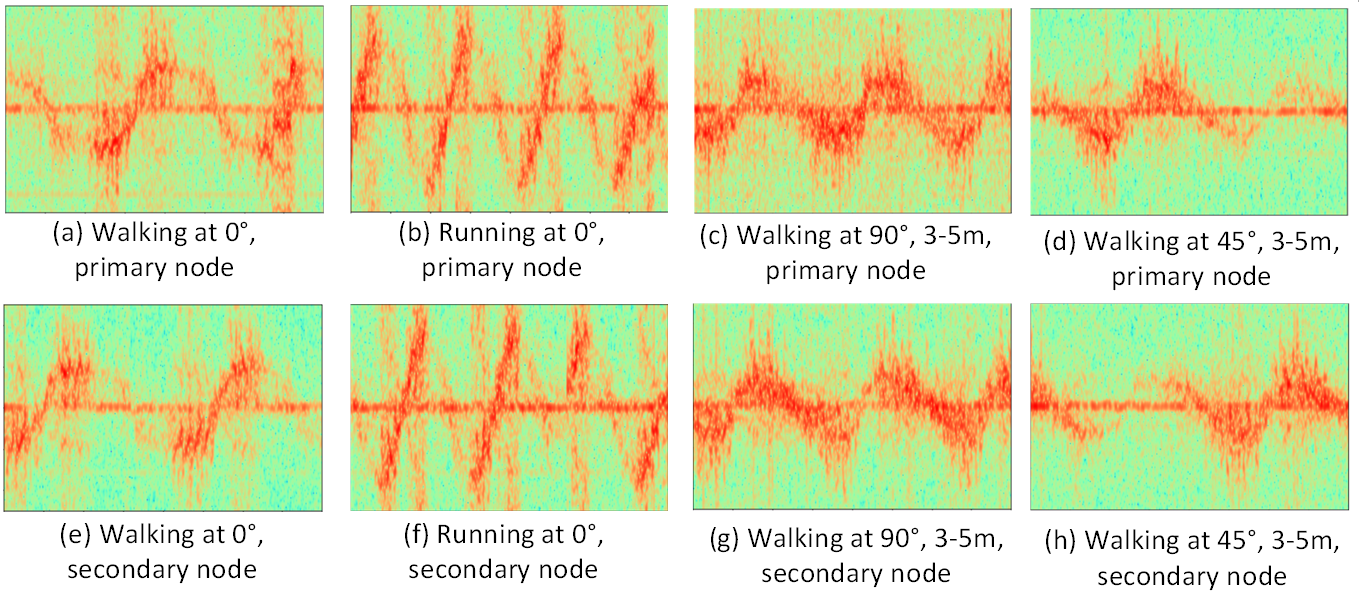
\includegraphics[width=3.7in]{ms_single}
\caption{Micro-Doppler signatures of an individual at different angles}
\label{fig_mss}
\end{figure}

The spectrograms in Fig. \ref{fig_ir9} represent the micro-Doppler signatures of an individual walking and running at \ang{90} in each one of the three ranges. As it can be seen, the patterns of the signal are different depending on the target’s distances to the primary node. The waveforms in Fig. \ref{fig_ir9}(a) and Fig. \ref{fig_ir9}(b) are smooth, the waveforms in Fig. \ref{fig_ir9}(c) and Fig. \ref{fig_ir9}(d) are more zigzagged, and the waveforms in Fig. \ref{fig_ir9}(e) and Fig. \ref{fig_ir9}(f) are discrete. The spectrograms of the secondary node are not shown, because the wave patterns collected by the secondary node in the range of 5-8m are similar to Fig. \ref{fig_ir9}(a) and Fig. \ref{fig_ir9}(b), the wave patterns in the range of 3-5m are similar to Fig. \ref{fig_ir9}(c) and Fig. \ref{fig_ir9}(d), and the wave patterns in the range of 1-3m are similar to Fig. \ref{fig_ir9}(e) and Fig. \ref{fig_ir9}(f). This indicates the distance does affect the wave pattern of the spectrograms of human activity.
\begin{figure}[!t]
\centering
%\captionsetup{justification=centering}
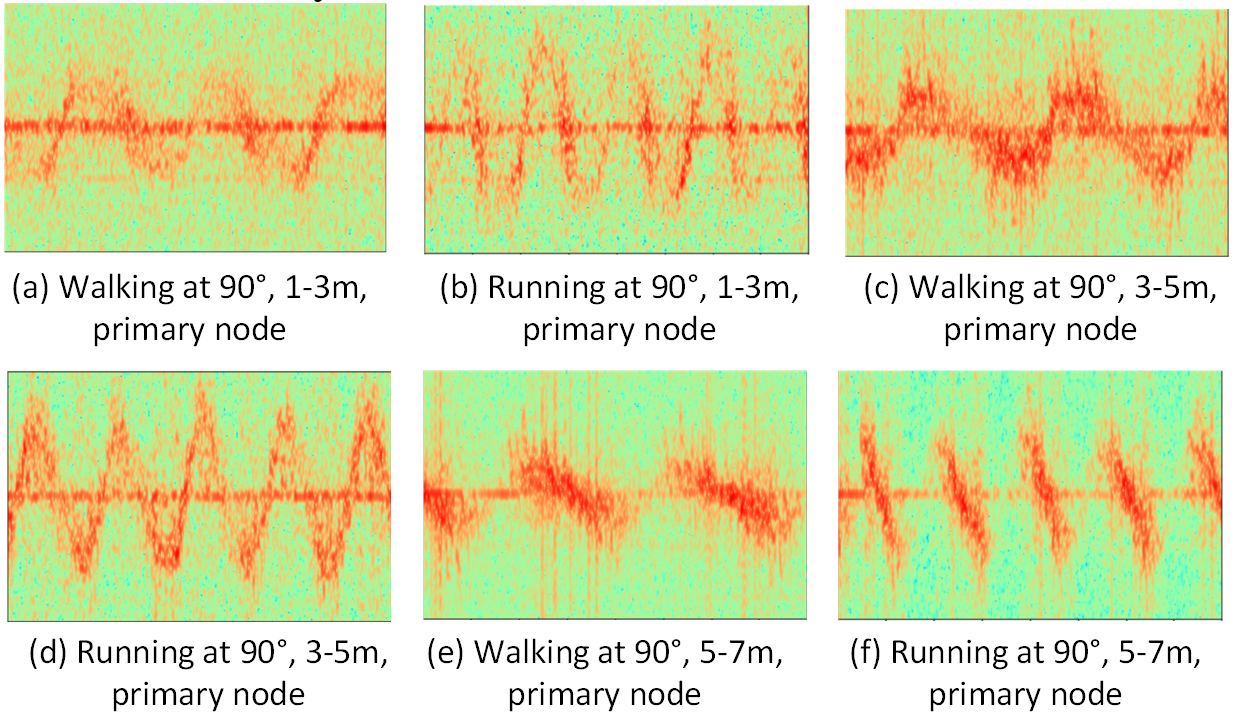
\includegraphics[width=3.5in]{individual_randar_90}
\caption{Micro-Doppler signatures of an individual walking and running in different ranges at \ang{90}}
\label{fig_ir9}
\end{figure}

Fig. \ref{fig_ir4} represents micro-Doppler signatures of an individual walking and running at \ang{45} in three different ranges. The patterns of these spectrograms are very similar to those of Fig.\ref{fig_ir9}, except that one part of each spectrogram is less clear, almost disappearing. This is because the target was not always in the detection range when he/she walked or ran back and forth at \ang{45}. Notice that the amplitude of the waves in Fig. \ref{fig_ir4} is a little smaller than in Fig. \ref{fig_ir9}.

\begin{figure}[!t]
\centering
%\captionsetup{justification=centering}
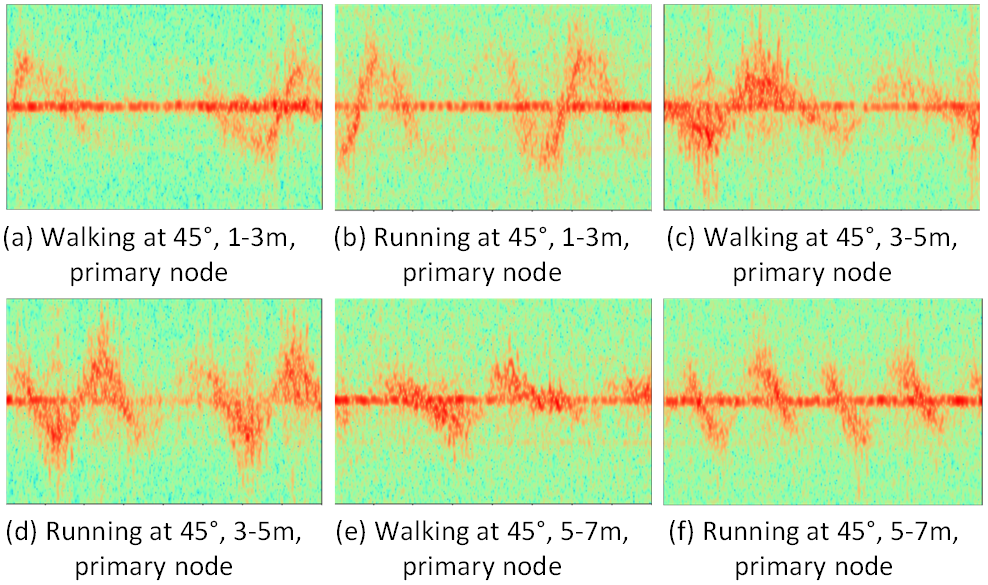
\includegraphics[width=3.5in]{individual_randar_45}
\caption{Micro-Doppler signatures of individual walking and running at \ang{45} with three different ranges}
\label{fig_ir4}
\end{figure}

\textit{Case 2: Activity classification and people counting in a group of people}: Nine individuals participated in this experiment, as shown in Fig. \ref{fig_ec}. Participants were arranged into three groups. The first group had two participants, the second group had three participants, and the third group consisted of four participants. Each group walked and ran in three ranges from three different angles (\ang{0}, \ang{45}, and \ang{90}) relative to the radar beam. Participants in the first or second group moved abreast. Participants in the third group were divided into two rows with two people in each row and they ran or walked at the same time inside the detection range. The main difference between \textit{Case 1} and \textit{Case 2} is the number of people that composed the target.
\begin{figure}[!t]
\centering
%\captionsetup{justification=centering}
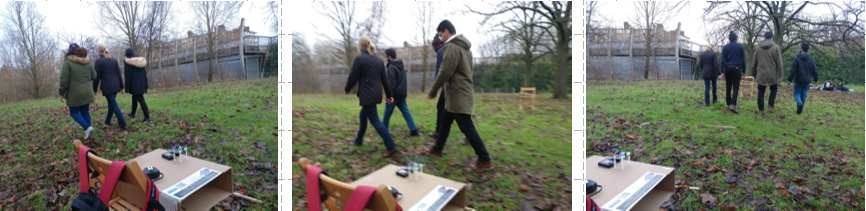
\includegraphics[width=3.5in]{ecounting}
\caption{Group behaviour classification and people counting}
\label{fig_ec}
\end{figure}

The spectrograms in Fig. \ref{fig_msc} show the micro-Doppler signatures of the target with different numbers of people. By the naked eye, it is difficult to find the visual differences among the spectrograms of different numbers of people. However, if we observe very carefully, it can be seen that the frequency waves in Fig. \ref{fig_msc}(c) and Fig. \ref{fig_msc}(d) are thicker than in Fig. \ref{fig_msc}(a) and Fig. \ref{fig_msc}(b). It could be understood that more people in a target would result in a more solid wave shape. However, this phenomenon cannot be observed in Fig. \ref{fig_msc}(e), Fig. \ref{fig_msc}(f), Fig. \ref{fig_msc}(g), and Fig. \ref{fig_msc}(h) possibly as a result of the speed of the movement. 
\begin{figure}[!t]
\centering
%\captionsetup{justification=centering}
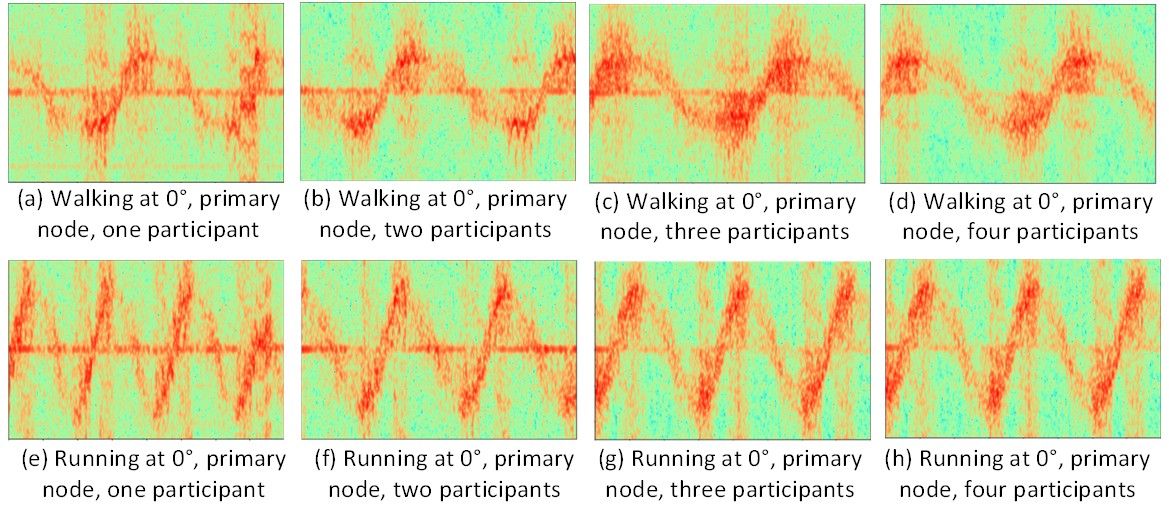
\includegraphics[width=3.7in]{mscounting}
\caption{Micro-Doppler signatures of different number of people}
\label{fig_msc}
\end{figure}

\textit{Case 3, differentiation between humans and dogs}: One human volunteer and two dogs participated in this experiment, as shown in Fig. \ref{fig_ani}. In the first experiment, separately, each dog was encouraged by their owners to move back and forth inside the detection range, in order to obtain micro-Doppler signatures of a dog only. In the second experiment, the volunteer walked a dog back and forth. Because it is hard to control the dog`’s speed (i.e. walk and run) inside the detection range, the experiment did not differentiate between walking and running, and only two angles (\ang{0} and \ang{90}) were investigated. Unavoidably, some noisy data was produced during the experiments, but the amount was small.  
\begin{figure}[!t]
\centering
%\captionsetup{justification=centering}
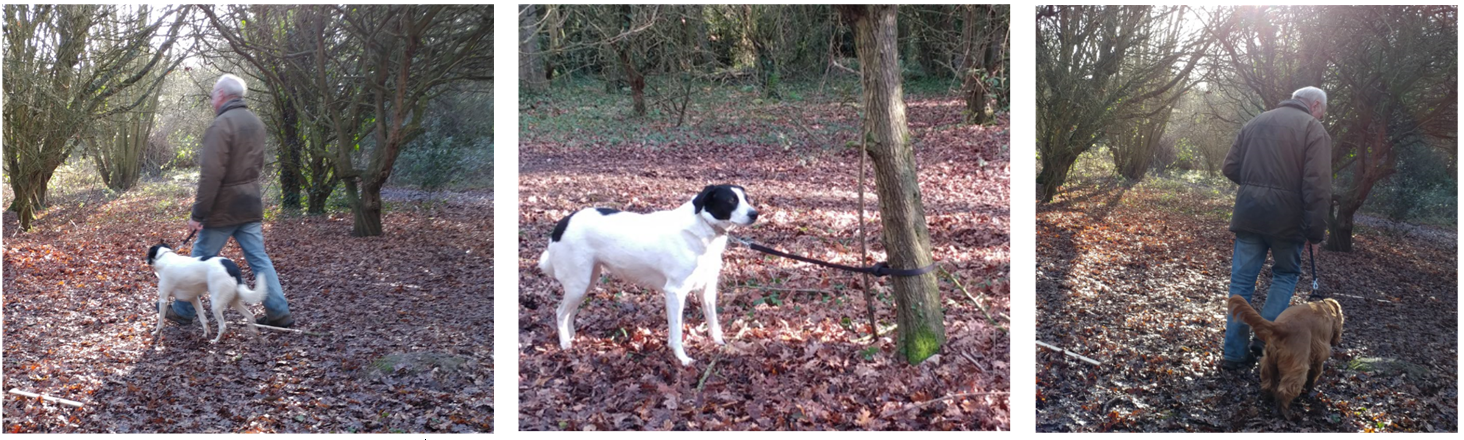
\includegraphics[width=3.6in]{animal}
\caption{Differentiation between humans and dogs}
\label{fig_ani}
\end{figure}

Combined with the data collected in \textit{Case 1} and \textit{Case 2}, all samples could be classified into 4 categories according to the different types of the targets, including human, dog, a person and a dog, and the background. As shown in Fig. \ref{fig_msani}, the spectrograms generated by different targets are different. Fig. \ref{fig_msani}(a) presents the periodic change of a human walking. Fig. \ref{fig_msani}(b) shows the micro-Doppler signatures of a moving dog. Visually, the frequency wave in Fig. \ref{fig_msani}(c) of a moving person and dog seems to have an overlapping shadow. The spectrogram of the scene background shown in Fig. \ref{fig_msani}(d) only contains a line around the frequency of 0Hz, this reflects the clutter in the environment around 0Hz. 
\begin{figure}[!t]
\centering
%\captionsetup{justification=centering}
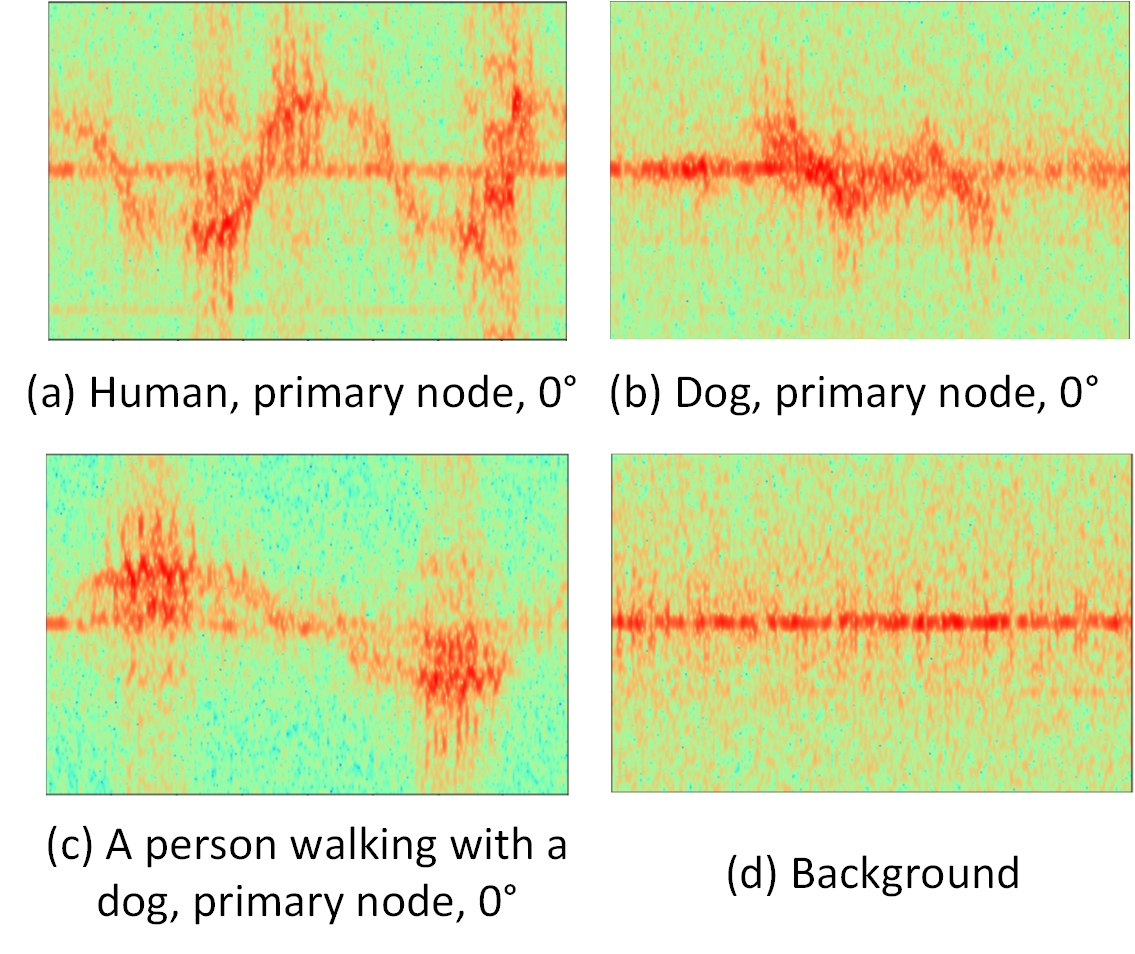
\includegraphics[width=3.4in]{msanimal}
\caption{Micro-Doppler signatures of different subjects}
\label{fig_msani}
\end{figure}

\section{Data Collection and preprocessing}
The data collected in the experiments requires further processing before feature extraction and classification are made. This section describes the process of data collection and data preprocessing in detail. Data preprocessing is needed in order to present the micro-Doppler signatures and attenuate the background noise.
\subsection{Data collection}
With the Doppler radar system described in Section II, radars signals were collected and stored in a database. As illustrated in Fig. \ref{fig_dfd}, signals collected by the BumbleeBee radars were transferred to the TelosB nodes and radio transferred to the TelosB base station. The TelsoB base station was connected to a computer which received the signals through a serial port. Finally, all data was stored into a MongoDB database system, which is an open source NoSQL database and it is usually utilized to store a large amount of time series data.
\begin{figure}[h]
\centering
%\captionsetup{justification=centering}
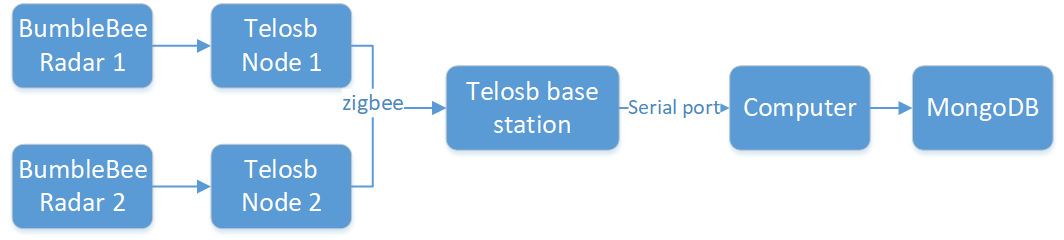
\includegraphics[width=3.4in]{dfd}
\caption{Data flow diagram of Doppler radar signals}
\label{fig_dfd}
\end{figure}

The final data stored into the database contains not only radar signals, but also labels that informed the time, the types of the target and the types of human activities (walking or running), etc. Table I shows the information of each field of a radar signal recorded in our MongoDB system. The sample frequency of the radars is 250 Hz. The data collected in the experiments were used to train the classifiers. In prediction, only the ID of the signals, I and Q values, and the time were used.
\begin{table}[]
\centering
\caption{Fields of the signal collection}
\label{tab_field}
\begin{tabular}{|l|l|}
\hline
\textbf{Field} & \textbf{Information}                                                                                                                           \\ \hline
ID             & The identity number of a Doppler radar signal                                                                                                  \\ \hline
Q              & The quadrature power value of a signal                                                                                                         \\ \hline
I              & The in-phase power value of a signal                                                                                                           \\ \hline
Time           & \begin{tabular}[c]{@{}l@{}}The time a signal was collected (accurate to a millisecond)\end{tabular}                                \\ \hline
SubjectType    & \begin{tabular}[c]{@{}l@{}}The type of a target or targets. `0` is human, `1` is dog, \\`2` is human and dog, `3` is no target.\end{tabular}  \\ \hline
SubjectID      & The ID of the targets.                                                                                                                         \\ \hline
SubjectNum     & The number of participants as a target.                                                                                                                     \\ \hline
Activity       & \begin{tabular}[c]{@{}l@{}}The type of human activity. `0` is walking,\\  `1` is running, `2` is no human activity\end{tabular}                \\ \hline
Angle          & \begin{tabular}[c]{@{}l@{}}The angle between the direction of human movement and\\ the radar beam.\end{tabular}                               \\ \hline
Range          & \begin{tabular}[c]{@{}l@{}}The range of the target located in. ‘0’ is 1-3m, \\ ‘1’ is 3-5m, ‘2’ is 5-8m, ‘3’ is not in any range.\end{tabular} \\ \hline
RadarNum       & \begin{tabular}[c]{@{}l@{}}The number of radars used in the system set up: 2.\end{tabular}               \\ \hline
NodeID         & \begin{tabular}[c]{@{}l@{}}The ID of primary node that consists of \\ BumbleBee 1 and Telsob 1 here.\end{tabular}                              \\ \hline
SecNodeID      & \begin{tabular}[c]{@{}l@{}}The ID of secondary node that consists of \\ BumbleBee 2 and Telsob 2 here.\end{tabular}                            \\ \hline
\end{tabular}
\end{table}

\subsection{Data preprocessing}
The original signal is a complex value ($I+jQ$). $I$ is the real part and $Q$ is the imaginary part. Micro-Doppler signatures are represented in a time-frequency domain. It is required to transform the original radar signals from the time-amplitude domain into the time-frequency domain using STFT. Fig. \ref{fig_dp}(b) shows a spectrogram generated by STFT. However, the spectrogram suffers from a band of heavy clutter between +/- 5 Hz. The clutter makes the fluctuations obtained from the human walking quite fade. In order to attenuate the clutter, a Butterworth high-pass filter is applied to the raw signals. The Butterworth high-pass filter can be represented by the following equation \cite{dogra2014image}:
\begin{equation}
\label{eq_butter}
\left | H(w) \right |^2=1/(1+(w/w_c )^{2n} )=1/(1+\varepsilon ^2 (w/w_s )^{2n} ),
\end{equation}
where $n$ is the order of filter, $w_c$ is the cutoff frequency (5 Hz here), $w_s$ is the stopband boundary frequency.

After filtering, a new spectrogram is generated as it can be seen in Fig. \ref{fig_dp}(c). The fluctuations obtained from human movements are now more distinctive. Note the spine of the plot corresponds to the motion from the torso, the smaller fluctuations around the spine corresponds to the motions from arms and legs. Positive and negative Doppler frequencies correspond to the subject moving toward or away from the radar, respectively. However, the high-pass filter is only used to attenuate parts of the clutter and noise that are below $w_c$. For improving the robustness of the classifiers, the samples are required to be collected from environments with high-levels of clutter. By training the classifiers with those samples, they can learn how to reduce the interference of the noise in the environment.
\begin{figure}[!t]
\centering
%\captionsetup{justification=centering}
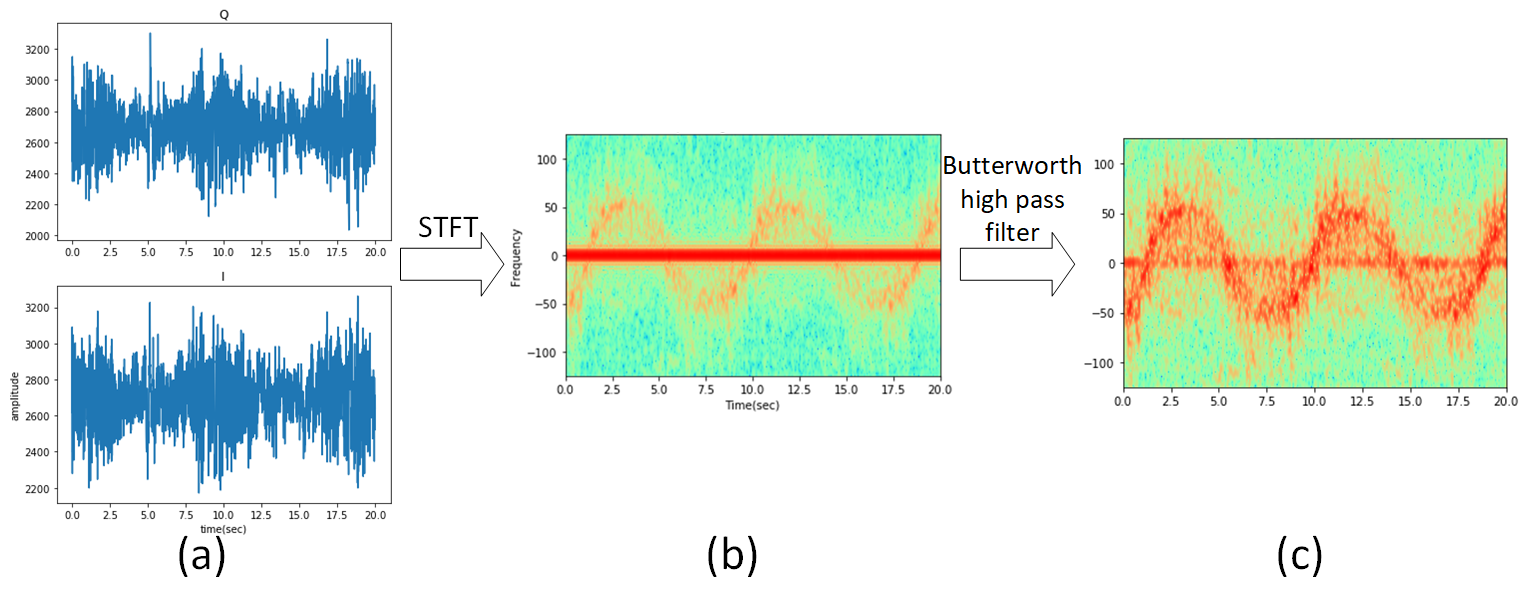
\includegraphics[width=3.4in]{data_processing}
\caption{Data preprocessing, (a) original signals, (b) spectrogram after STFT, (c) spectrogram after high-pass filter}
\label{fig_dp}
\end{figure}

With the STFT technique, a different length of a sequence will result in a different width of the frequency spectrogram. A windowed short time FFT processing technique with a window length of 64 samples and a Hanning weighting, transforms a sequence of 2500 signal samples into a frequency spectrogram with the size of $2048\times 304\times 1$ (2048 is the height, 304 is the width, 1 is the depth). The frequency spectrogram can be taken as an image with one channel. Fig. \ref{fig_sliding} presents a frequency spectrogram that was created from a sliding-window with the window size of 2500 frames (2500 samples within the sliding window) and the sliding step with the length of 100 frames. The sampling frequency of the micro-Doppler signals is 250Hz. So by moving the sliding-window with continuous sliding steps, a spectrogram can be extracted at every 0.4 seconds, which is calculated by $(Sliding\; step \;length)/(sample\; frequency)$, i.e. $100/250$. The effect of the window size is investigated in Section IX.
\begin{figure}[!t]
\centering
%\captionsetup{justification=centering}
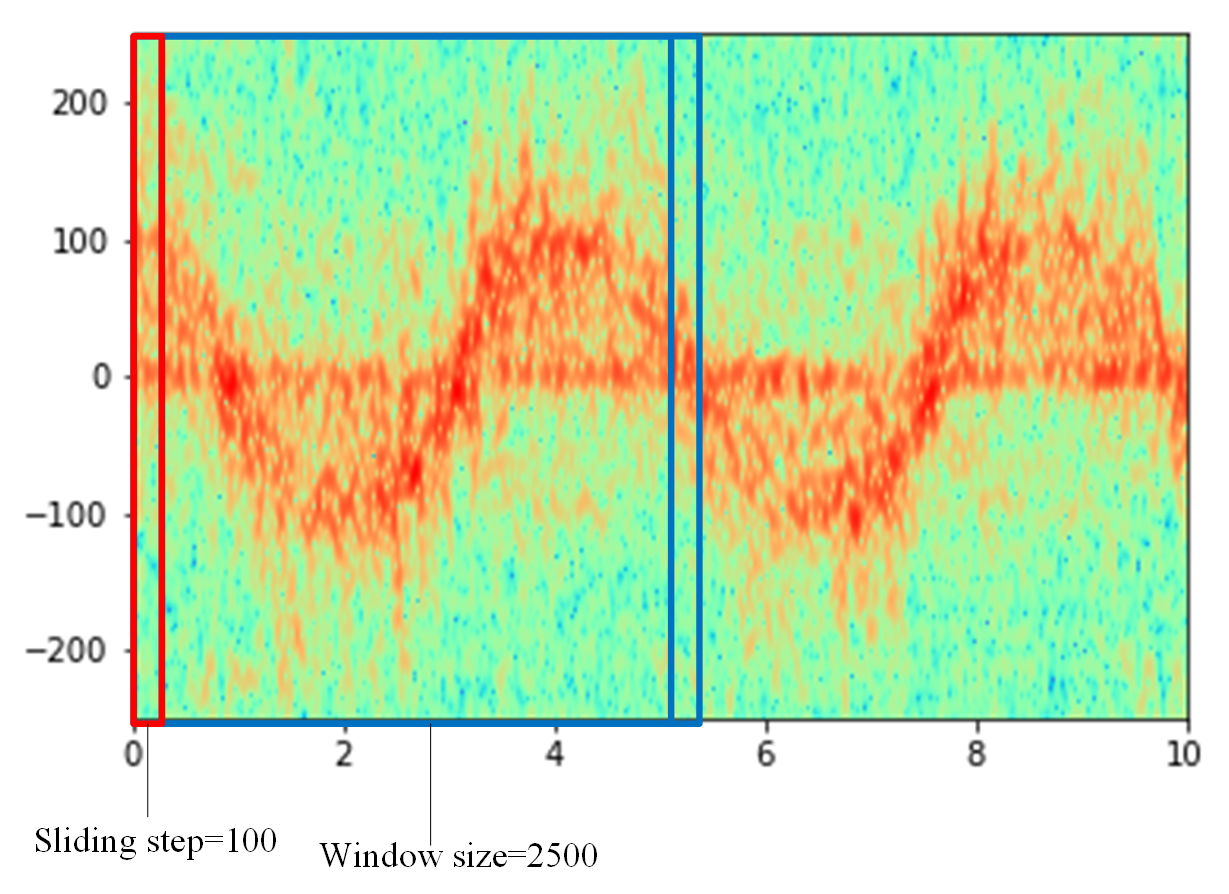
\includegraphics[width=3.4in]{sliding}
\caption{A sliding window of STFT}
\label{fig_sliding}
\end{figure}

Through the above processing methods and using an STFT sliding window of 1250 frames (time length of 5s), the described experiments generated 46900 spectrograms in total. The composition of the samples/spectrograms is shown in Table \ref{tb-sample}.
% Please add the following required packages to your document preamble:
% \usepackage{multirow}
\begin{table}[]
\centering
\caption{The composition of samples}
\label{tb-sample}
\begin{tabular}{|c|c|c|c|c|}
\hline
\textbf{Subject}               & \textbf{Angle} & \textbf{Walking} & \textbf{Running} & \textbf{Total}         \\ \hline
\multirow{3}{*}{Single person} & 0°             & 1150             & 1200             & \multirow{3}{*}{15400} \\ \cline{2-4}
                               & 45°            & 2700             & 3150             &                        \\ \cline{2-4}
                               & 90°            & 3500             & 3700             &                        \\ \hline
\multirow{3}{*}{Two people}    & 0°             & 550              & 550              & \multirow{3}{*}{7000}  \\ \cline{2-4}
                               & 45°            & 1600             & 1550             &                        \\ \cline{2-4}
                               & 90°            & 1150             & 1600             &                        \\ \hline
\multirow{3}{*}{Three people}  & 0°             & 600              & 550              & \multirow{3}{*}{7200}  \\ \cline{2-4}
                               & 45°            & 1250             & 1700             &                        \\ \cline{2-4}
                               & 90°            & 1300             & 1800             &                        \\ \hline
\multirow{3}{*}{Four people}   & 0°             & 500              & 550              & \multirow{3}{*}{6950}  \\ \cline{2-4}
                               & 45°            & 1200             & 1650             &                        \\ \cline{2-4}
                               & 90°            & 1150             & 1900             &                        \\ \hline
Dog                            & 90°            & \multicolumn{2}{c|}{1350}           & 1350                   \\ \hline
\multirow{2}{*}{Human and Dog} & 0°             & \multicolumn{2}{c|}{1200}           & \multirow{2}{*}{3150}  \\ \cline{2-4}
                               & 90°            & \multicolumn{2}{c|}{1950}           &                        \\ \hline
Background                     & \multicolumn{3}{c|}{}                                & 5850                   \\ \hline
\end{tabular}
\end{table}


For the classification, the samples were separated into two groups, 80\% of the samples were used for training and validation, and 20\% for testing. As it can be seen from Table \ref{tb-sample}, the sample size for the classes is not balanced. In order to overcome this problem, different weights were assigned to each class in the training process; and the weight ratio was inversely proportional to the proportion of spectrograms of the various classes. However, for human recognition, because the numbers of spectrograms of the experiments with humans and the background are far greater than the number of spectrograms of the experiments with a dog (including human and dog), we randomly selected 2000 spectrograms of human and 2000 spectrograms of the background for the training.

In the training process, a 10-fold cross-validation has been applied; the samples/spectrograms for training and validation are further split randomly into 10 subsets without replacement. In each training iteration, nine subsets are used for training and one subset is used for validation.

\section{Feature Extraction Using Two-Directional Two-Dimensional Principal Component Analysis}
The time-frequency spectrogram is a form of representation of the micro-Doppler signatures. It presents the characteristics of human activity in the time-frequency domain. Feature extraction in micro-Doppler analysis is used to reduce the number of features of a spectrogram; the aim is to identify features of the signal, which are required for recognizing an activity, and to disregard other parts as background noise. A good feature extraction technique is a very important component in a recognition system; because those extracted features will be fed into the classification algorithms and this will dictate the quality of the classification and the time that the classifiers will take to sufficiently train the model. For classifying different activities, it is required to extract features from the spectrograms and use these features to train the machine learning algorithms, such as SVM, and \textit{k}NN to differentiate the activities.

Two-directional Two-dimensional Principal Component Analysis was firstly developed by \cite{zhang20052d} and used for face representation and recognition. The authors of \cite{tivive2013image} applied 2D2PCA for micro-Doppler features extraction and compared it with Gabor Wavelet Filter, Mel-frequency Cepstral Coefficients, Cadence Frequency based method, and Empirical Mode Decomposition. The performance of 2D2PCA exceeded all the others significantly, which is the reason why it is used in this research.

PCA is well-known as a classic feature extraction and dimensionality reduction technique \cite{wold1987principal}. A spectrogram is an image composed of a two-dimensional structure of pixels. In order to use PCA, firstly the two-dimensional image of the spectrogram must be transformed into a one-dimensional vector. 2D2PCA can be regarded as a two-dimensional version of the PCA, 2D2PCA performs feature extraction on the rows and columns of an image simultaneously and it is more efficient in computing the covariance matrices, the eigenvalues and the eigenvectors than PCA alone.

A spectrogram generated by STFT can be denoted by a matrix $A\in R^{m \times n}$, where $R$ indicates  that the elements of A consist entirely of real numbers. Let  $X\in R^{n\times d},n \geq d$ be a projection matrix with orthonormal components. $Y\in R^{m\times d}$ is generated by projecting $A$ onto $X$, which can be written as $Y=AX$. The reduction of the dimensionality is achieved by the selection of a suitable value for $d$, which decides how many features will be kept in each row, also is the final number of columns after the projection.   

Matrix $Y$ must preserve relevant information of the specific activity contained in the spectrogram. An ideal projection matrix should ensure that the result after the projection is very distinct from others of different activities. This makes the samples of different activities more independent to each other so that they do not cluster together. Therefore, it is beneficial to the classification if the most relevant information is kept after projection. In order to determine a good projection matrix $X$, the following criterion \cite{zhang20052d} is adopted:
\begin{equation}
\label{eq:llk}
\begin{split}
&J(X)=trace\{E[(Y-EY) (Y-EY)^T ]\} \\&=trace\{E[(AX-E(AX))(AX-E(AX))^T ]\}\\&=trace\{X^T E[(A-EA)^T (A-EA)]X\},
\end{split}
\end{equation}
where $J(\cdot)$ is an objective function. In order to find the optimal projection matrix X, it is required to maximize $J$. $E$ is the expectation operator that when applied to a matrix produces a new matrix containing the expected values of the elements of the original matrix. The last term in Eq. (\ref{eq:llk}) follows the commutative property of matrices where $trace(QP)=trace(PQ)$, $Q$ and $P$ represent any two matrices. 

The covariance matrix \cite{zhang20052d} of $A$ is defined as:
\begin{equation}
G=E[(A-EA)^T (A-EA)], 
\end{equation}
Suppose that the training set consists of $M$ spectrograms $\{A_1,A_k,\ldots,A_M\}$, the covariance matrix  $G$ can be computed as:
\begin{equation}
G=(1/M) \sum_{k=1}^{M}〖(A_k-\bar{A})^T (A_k-\bar{A})〗,
\end{equation}
where $\bar{A}$ is the average spectrograms as $\bar{A}=(1/M) \sum_{k=1}^{M}A_k$.
Eq. (\ref{eq:llk}) can be simplified as:
\begin{equation}
J(X)=X^T GX,
\end{equation}
Let $A_k=〖[(A_k^{(1)} )^T (A_k^{(2)} )^T\ldots〖(A_k^{(m)})〗^T]〗^T$ and $\bar{A} ̅=〖[(\bar{A}^{(1)} )^T (\bar{A}^{(2)} )^T\ldots〖(\bar{A}^{(m)})〗^T]〗^T$, where $A_k^{(i)}$ and $\bar{A}^{(i)}$ denote the $i_{th}$ row of $A_k$ and the $i_{th}$ row of $\bar{A}$, respectively. The covariance matrix  $G_r$ can be rewritten as:
\begin{equation}
G_r=(1/M) \sum_{k=1}^{M}\sum_{i=1}^{m}〖(A_k^{(i)}  -\bar{A}^{(i)} )^T (A_k^{(i)}  -\bar{A}^{(i)})〗,
\end{equation}

The covariance matrix $G_r$ is essentially the same as $G$, the only difference is that matrix $A$ is taken as a set of row vectors. Through diagonalization of covariance matrix $G_r$, the ideal projection matrix $X$ can be obtained.

In the same way, matrix $A$ also could be taken as a set of column vectors. Let $A_k=[(A_k^{(1)} )(A_k^{(2)})\ldots(A_k^{(n)})]$ and $\bar{A}=[(\bar{A}^{(1)})(\bar{A}^{(2)} )\ldots(\bar{A}^{(n)})]$, where $A_k^{(j) }$ and $\bar{A}^{(j)}$ denote the $j_{th}$ column of $A_k$ and the $j_{th}$ column of $\bar{A}$, respectively. The covariance matrix  $G_c$ could be rewritten as:
\begin{equation}
G_c=(1/M) \sum_{k=1}^{M}\sum_{j=1}^{n}〖(A_k^{(j)}  -\bar{A}^{(j)} ) (A_k^{(j)}  -\bar{A}^{(j)})^T〗,
\end{equation}

Let $Z\in R^{m \times q}$ be a matrix with orthonormal columns.  Projecting matrix $A$ onto $Z$ yields matrix $B=Z^T A,B\in R^{q \times n}$. The reduction of the dimensionality is achieved by the selection of a suitable value for $q$, which determines how many features will be kept in each column, it also corresponds to the number of rows of $B$. $Z$ can be obtained through diagonalization of $G_c$.

After the projection matrices $X$, $Z$ are obtained, $A$ must be projected onto $X$ and $Z$ simultaneously in order to yield a matrix $C$:
\begin{equation}
C=Z^T AX,
\end{equation}
the matrix $C$ is called the \textit{coefficient matrix}. It can be taken as the input features that are fed into SVM and $k$NN classifiers.
\begin{figure}[!t]
\centering
%\captionsetup{justification=centering}
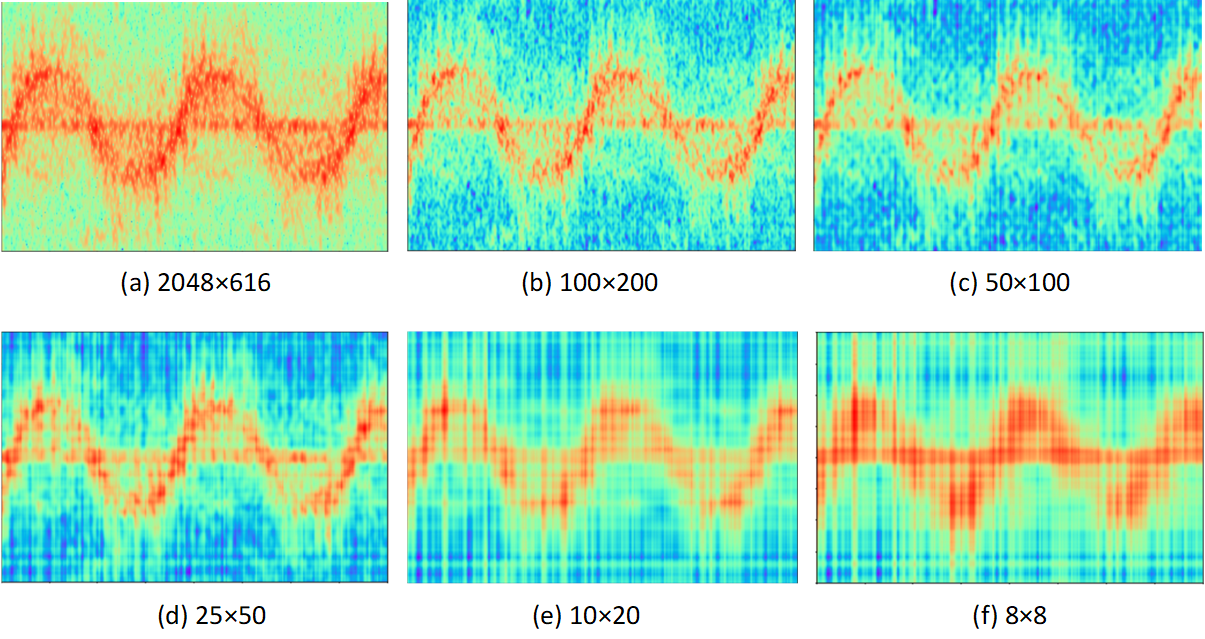
\includegraphics[width=3.6in]{pca2d2}
\caption{Dimensionality reduction with 2D2PCA}
\label{fig_tf}
\end{figure}

Fig. \ref{fig_tf}(a) is a spectrogram whose size is $2048\times 616$ pixels. It is the result of an echoed radar signal of a human walking indoors. The method 2D2PCA was applied on this original spectrogram for different row and column dimension reductions. The results are shown in Fig. \ref{fig_tf}(b) and Fig. \ref{fig_tf}(c). We note that Fig. \ref{fig_tf}(b) and Fig. \ref{fig_tf}(c) still retain detailed time-frequency characteristics (the periodic waves), but the image dimensions are well reduced, visually they are almost the same as the original spectrogram. Even when reducing the dimensionality to 8 rows and 8 columns the remained characteristics still can reflect the periodic trend of a human walking as it can be seen in Fig. \ref{fig_tf}(f). 2D2PCA is able to keep most of the distinctive features (pixels) while greatly reducing the dimensions of the micro-Doppler signatures.

\section{Machine learning models}
Three classifiers, including CNN, SVM, and \textit{k}NN were modeled in this work. All the three classifiers were modeled to classify the samples for different classification outputs. This section details how the classifiers were built and what hyper-parameters were used and optimized.
\subsection{Convolutional neural network}
Deep learning has been applied to many research areas and has achieved quite remarkable results. CNNs are widely used in image recognition and classification due to their power of automatically learning hierarchical representations directly from the raw data input. In this research, each spectrogram can be considered as an image with one channel. So a CNN is suitable to be applied into human recognition and activity classification using the spectrograms.

CNNs are a variant of artificial neural networks because they present a hierarchical sequence of convolutional layers alternated by pooling layers before the fully-connected layer of a regular neural network. A convolutional layer allows the network to detect spatial patterns over different parts of the input, and a pooling layer to learn translational invariance of the input. A typical CNN is depicted in Fig. \ref{fig_cnn}, where the \textit{Input} represents the dataset the network takes in, the \textit{Convolution} and \textit{Subsampling} (pooling function) are the operations performed on the data, the \textit{Feature maps} are the intermediate set of outputs; and the \textit{Output} is the final set of outputs. The unique architectural configuration of a CNN is defined by its \textit{hyperparameters}, whose values are set before the network is trained. An instance of a convolutional network is defined by its parameters whose values are learned during the network training \cite{bergado2018recurrent}.
\begin{figure}[!t]
\centering
%\captionsetup{justification=centering}
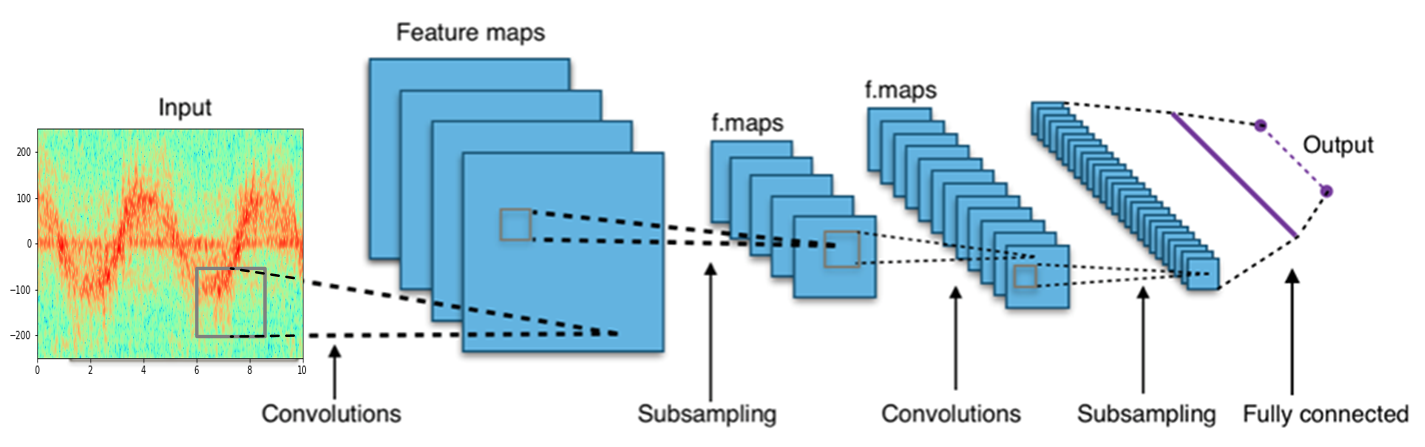
\includegraphics[width=3.6in]{cnn}
\caption{The structure of a CNN}
\label{fig_cnn}
\end{figure}

The next subsections describe details of the input, operations, and the output of a CNN making reference how it is applied to micro-Doppler signatures. We also detail how training and regularization are performed. Finally, we describe our proposed CNN architecture, called RadarNet, to perform the classification of the micro-Doppler signatures.
\subsubsection{Input}
The input in a CNN can be a full image or a set of it \cite{bergado2018recurrent}. An image is defined by its size, which is the height (number of rows) and width (number of columns) of its array of pixels and the number of channels ($C$) that are the different colors of the pixels (red, green and blue). Assuming $N$ is the number of images processed in parallel by the network and the image size as $H\times W$, a CNN input could be defined as an array $N\times H\times W\times C$. As described in section IV, a sequence of 2500 signal samples of one radar is transformed into a frequency spectrogram with the size of $2048 \times 304 \times 1$ (2048 is the height, 304 is the width, 1 is the depth), therefore the frequency spectrogram can be taken as an image with one channel.

\subsubsection{Operations}
A \textit{convolutional layer} is the main fundamental layer of a CNN. Each convolutional layer performs an aggregational operation aimed to learn the feature representation of the input (in our case spectrograms) and reduce the number of learnable parameters; it operates on the input/feature maps by applying a filter (e.g. kernel function) over the input. A convolution applies a linear operation on the input/feature maps using a set of filters $F$. The filter size is a matrix $G\times G$ of learnable parameters, on an input feature map $x$, it produces an output feature map $x^{'}$ as
\begin{equation}
\begin{split}
x^{'}=\sum_{i=1}^{k}\sum_{r=1}^{G}\sum_{c=1}^{G}x_{rc}\cdot F_{i}+b^{'}
\end{split}
\end{equation}
where $k$ is the number of filters $F$, $b^{'}$ is the bias parameter associated with the feature map $x^{'}$.

By convolving the input with the filter, a set of feature maps is produced. A convolutional layer is parameterized by a \textit{depth}, a \textit{kernel field size}, a \textit{stride}, and a \textit{zero-padding}. The depth determines the channel size of the output (i.e. the desired number of feature maps). The kernel field size, i.e. the filter size, covers a small region of pixels of the input image at each convolution step (see the red square in Fig. \ref{fig_convol}). Each element in a feature map is generated by the filter convolving with the covered region of the input (e.g. the generated elements in the yellow feature map in Fig. \ref{fig_convol}). The stride determines the number of pixels by the filter which is moved during each filtering step over the image. As can be seen in Fig. \ref{fig_convol} by the red and purple squares (representing the filter) over the Input image. The zero-padding is used to pad the input with zeros on its border, as seen in Fig. \ref{fig_convol}. The zero-padding is useful to determine a desired output size of the feature map. For example, given an input image of height and width  $H\times W$, a kernel field size of $G\times G$, a stride $S$, and an amount of zero padding $P$, the spatial size ($H{'}\times W{'}$) of the feature map generated can be computed as  \cite{bergado2018recurrent}: 
\begin{equation}
\begin{split}
H{'}=(H-G+2P)/S+1,\\
W{'}=(W-G+2P)/S+1
\end{split}
\end{equation}


Fig. \ref{fig_convol} provides a numerical example of the convolution process: assuming an image with the size of $4\times 4$ pixels that is zero-padded with value $1$, then convolutionalized by a kernel of $3\times 3$ with a stride of $2$, a resulting feature map of $2\times 2$ neurons is produced.  
\begin{figure}[!t]
\centering
%\captionsetup{justification=centering}
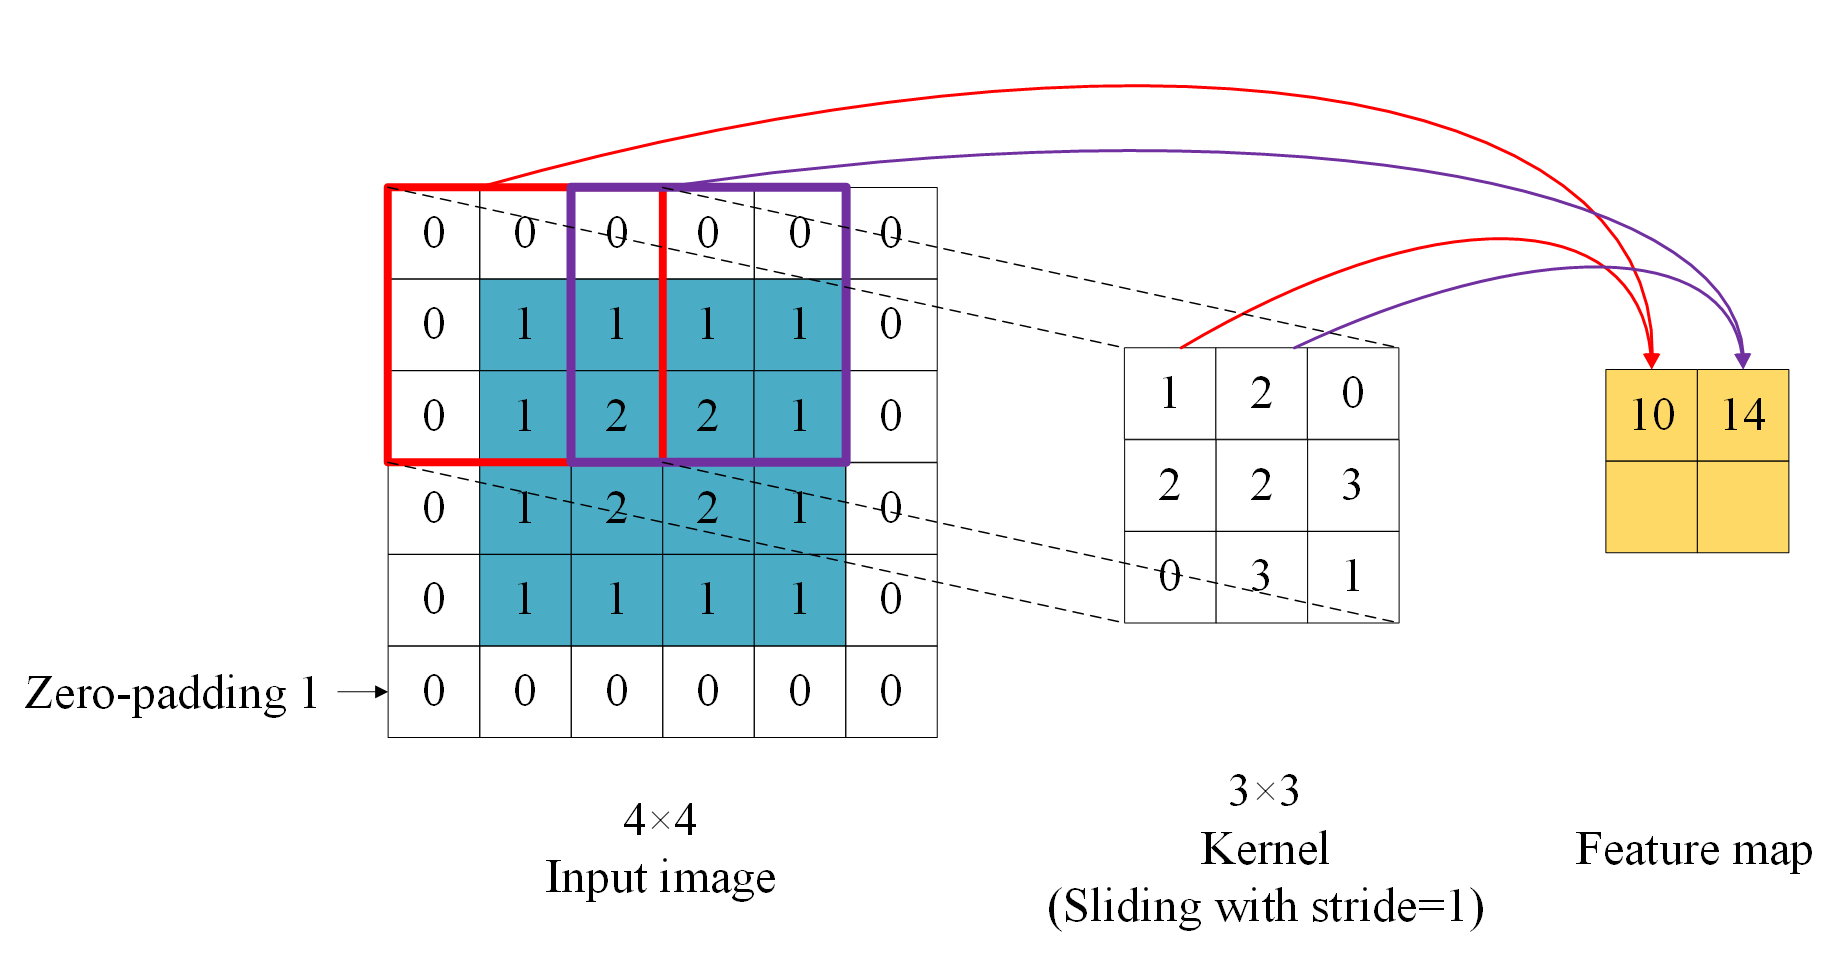
\includegraphics[width=3.6in]{convolution}
\caption{Convolution process}
\label{fig_convol}
\end{figure}

The \textit{pooling layer} is a form of non-linear down-sampling. It is designed to reduce the spatial size (dimensionality) of the input, in order to reduce the number of parameters (e.g. neurons and their connectivity) in the CNN. It aggregates the values of a local region of the input (window), commonly by applying an average or a maximum function.  Max pooling is the most common function to implement pooling by using the maximum function. It partitions the input image into a set of non-overlapping windows (e.g. the red bordered square in Fig. \ref{fig_pool}). For each such window, it takes the maximum neuron value of that window and places it as an output neuron (as shown in Fig. \ref{fig_pool}, where the resulting maximum value is 8 of the bordered red square). It is common to periodically insert a pooling layer between successive convolutional layers in a CNN architecture.  A complete Max-pooling operation is shown in Fig. \ref{fig_pool} for an input matrix of $4\times 4$ that is reduced to a $2\times 2$ matrix size, by using a $2\times 2$ sliding window and taking the maximum value of each window.
\begin{figure}[!t]
\centering
%\captionsetup{justification=centering}
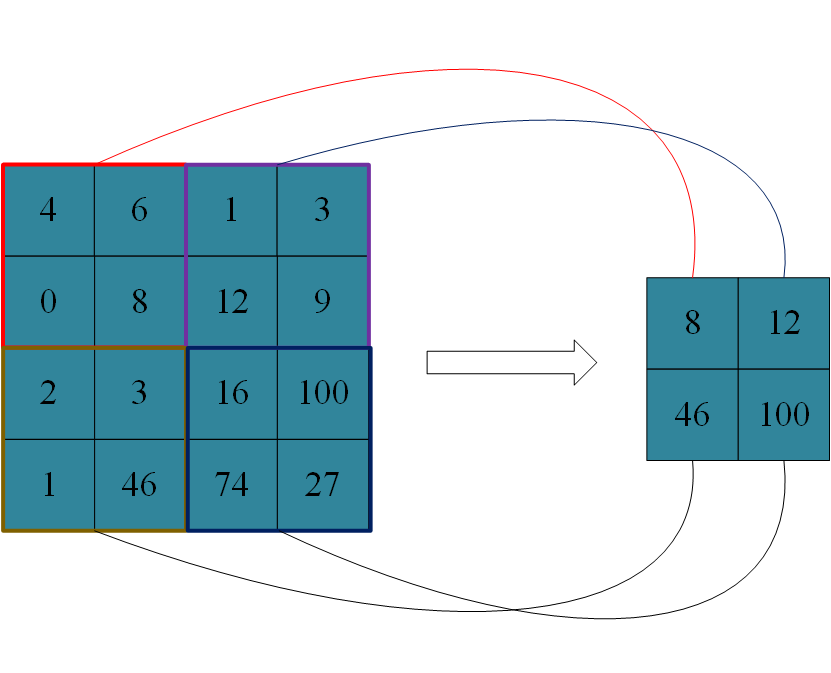
\includegraphics[width=2.6in]{pooling}
\caption{Max-pooling operation}
\label{fig_pool}
\end{figure}

\textit{Fully connected layers} can be seen as regular neural network layers. All neurons in the previous layer are transformed into a one-dimensional vector in a fully connected layer. Fully connected layers are added after all convolutional layers and pooling layers.

An \textit{activation layer} is not a typical layer in CNNs, but it is a nonlinearity operation commonly used in neural networks. It increases the nonlinear properties of CNNs. As the result of a series of linear operations (like convolutions) can be a single-linear operation, an elementwise nonlinear function can be applied between convolutions in order to introduce nonlinearity \cite{bergado2018recurrent}. This makes CNNs capable to learn more complex mappings of input to output. The activation function used in our work is the ReLU (Rectified Linear Units) \cite{nair2010rectified}, which is formulated as:
\begin{equation}
f(x)=Max(0,x),
\end{equation}
Other functions are also used to increase nonlinearity, such as
\begin{equation}
\begin{split}
\text{sigmoid}: f(z)=1/(1+\exp(-z) ),\\
\text{tanh}: f(z)=\tanh(z)=\frac{e^z-e^{(-z)}}{e^z+e^{(-z)}}
\end{split}
\end{equation}

ReLU is often preferred over other functions because it trains the neural network several times faster without a significant penalty to the generalization accuracy.
\subsubsection{Output}
The Feature maps are intermediary outputs of a CNN layer and at the same time input to the next layer. In CNNs, the final outputs comprise of final score maps, which represent the probabilities of each input element belonging to a label. The calculated accuracy is in relation to the final score maps and the reference labels.
\subsubsection{The Network Training Process}
The model is trained to minimize an objective function in terms of the parameters of the network. For a given classification, let $C$ be the number of labeled classes, the following cross-entropy loss function \cite{de2005tutorial} is often used:
\begin{equation}
E_y (y^{'} )=-\sum_{i=1}^{N}y_i\cdot log(y_i^{'})
\end{equation}
where $E$ is the loss function evaluated over $N$ samples, $y_i$ is the original label of the $i_{th}$ sample and $y_i^{'}$ is the class score maps of a sample $i$ calculated using a \textit{softmax} activation function \cite{dunne1997pairing}:
\begin{equation}
y_j=exp(x_j)/(\sum_{c=1}^{C}exp(x_c))
\end{equation}
where $y$ is the softmax score and $x$ is the output layer containing unnormalized class scores.

In order to minimize the objective function, a backpropagation with gradient descent is normally applied. Computing the gradient yields to:
\begin{equation}
\partial E/\partial y_i =-y_i^{'}/y_i 
\end{equation}
\begin{equation}
\begin{split}
\partial y_i/\partial x_k&=\left\{\begin{matrix}
\frac{e^{x_i}}{\sum_{c=1}^{C}e^{x_c}}-(\frac{e^{x_i}}{\sum_{c=1}^{C}e^{x_c}})^2 & i=k\\ 
-(\frac{e^{x_i}e^{x_k}}{\sum_{c=1}^{C}e^{x_c}})^2
& i\neq k
\end{matrix}\right. \\
&=\left\{\begin{matrix}
y_i(1-y_i)) &i=k \\ 
 -y_iy_k& i\neq k
\end{matrix}\right.
\end{split}
\end{equation}
\begin{equation}
\begin{split}
\partial E/\partial x_i&=\sum_{k=1}^{C}(\partial E/\partial y_k)(\partial y_k/\partial x_i) \\&=
\frac{\partial E}{\partial y_i} \frac{\partial y_i}{\partial x_i}-\sum_{k\neq 1}^{C}\frac{\partial E}{\partial y_k}\frac{\partial y_k}{\partial x_i}\\&=-y_i^{'}(1-y_i)+\sum_{k\neq 1}y_k^{'}y_i\\&=-y_i^{'}+y_i\sum_{k\neq 1}y_k^{'}\\&=y_i-t_i
\end{split}
\end{equation}

Then the partial derivative of the loss function with respect to convolutional kernels $w_{ji}$ connecting input unit $i$ to the hidden units in the top layer, indexed by $j$, has a gradient of
\begin{equation}
\partial E/\partial w_{ij}=\sum_{i=1}^{C}(\partial E/\partial x_i)(\partial x_i/\partial w_{ij})=(y_i-t_i)h_i
\end{equation}
For units $j$ in the hidden layer, we have
\begin{equation}
\begin{split}
\partial E/\partial x_{j}&=\sum_{i}(\partial E/\partial x_i)(\partial x_i/\partial h_j)(\partial h_j/\partial x_j)\\ &=\sum_{i=1}^{C}(y_i-t_i)(h_i(1-h_i))
\end{split}
\end{equation}

The iterative training rule for updating the network parameters $w_{ji}$ and hidden units $j$ through the gradient descent strategy is as follows:
\begin{equation}
\begin{matrix}
w_{ij}\leftarrow w_{ij}-\alpha \cdot (\partial E/\partial w_{ij})\\ 
x_j\leftarrow x_j-\alpha \cdot (\partial E/\partial x_{j})
\end{matrix}
\end{equation}
where $\alpha$ is the learning rate for the whole network, it is a hyperparameter that is required to be initialized before the training.

\subsubsection{Regularization of CNNs}
Regularization are techniques used to address the problem of overfitting in statistical models. Overfitting occurs in deep learning when a CNN model classifies with high accuracy during training but presents poor classification accuracy in unseen test data. Overfitting is normally due to the rare dependencies in the training data that may not occur in the overall population.  The most common regularization methods are: \textit{data augmentation, early stopping, dropout and weight decay}. \textit{Data augmentation} increases the number of training samples by introducing distortions in the original samples by permuting samples or applying translational transformations. The amount of distortion should still ensure the labelling of each new training sample is still valid, this allows a model to become more invariant to small changes in input and hence allow for better generalization of the CNN. \textit{Early stopping} is to stop the training process by monitoring the loss on the validation set in order to prevent the overfitting resulted by over-training. When the validation loss increases for a specified number of iterations, the training is stopped. \textit{Dropout} \cite{srivastava2014dropout} is a regularization method commonly used in neural networks. The term ``dropout`` refers to dropping out a part of the units in a neural network. By avoiding training all nodes on all training data, dropout decreases overfitting in neural networks. \textit{Weight decay} adds a penalty term by multiplying each weight in the gradient descent at each epoch with a factor $\lambda 
,(0<\lambda 
<1)$, in order to penalize large weights. With weight decay term, the $w_{ij}$ in 
\begin{equation}
w_{ij}\leftarrow w_{ij}-\alpha \cdot (\partial E/\partial w_{ij})-\alpha \cdot \lambda  w_{ij}
\end{equation}

\subsubsection{RadarNet – Our Proposed CNN}
Our radar system consists of two BumbleBee radars. Both of them detect the target at the same time. In order to fuse the signals from the radars, the spectrograms generated from them are firstly downsampled into the size of $50\times 50\times 1$, then overlapped together. The downsampling is achieved by resizing the spectrograms using bilinear interpolation algorithm. It is beneficial to accelerate the training phrase by reducing the number of parameters since the size of $2048\times 304\times 1$ is too large. The resulting overlapped spectrograms can be considered as images with two channels. As shown as Fig. \ref{fig_cnn_}, the overlapped spectrogram with the shape of $50\times 50\times 2$ is input into a CNN model, which is named `RadarNet`. RadarNet contains three convolutional layers (C1, C2, and C3), two Max Pooling layers (M1, M2) and two fully connected layers. All three convolutional layers use $3\times 3$ kernels to do the convolutionalization. The C1 layer contains $16$ feature maps, and the size of each feature map is $48\times 48\times 1$. A $2\times 2$ filter is used to perform the \textit{Max Pooling} on C1, and generate the M1 layer. The C2 layer contains $32$ feature maps, and the size of each feature map is $22\times 22\times 1$. The resulting M2 layer by Max-Pool the C2 layer has the size of $11\times 11\times 1$. The C3 layer contains 48 feature maps, each feature map is a $9\times 9\times 1$ matrix. The F1 layer contains 356 hidden units, and the F2 contains 160 hidden units.

In RadarNet, Dropout has been used to control overfitting with an initial dropout rate of 0.4. Batch normalization \cite{ioffe2015batch} has been applied on $M1$, $M2$, $F1$, and $F2$ as a regularizer to accelerate convergence. Batch normalization normalizes the output of a previous activation layer by subtracting the batch mean and dividing by the batch standard deviation. The Batch normalization is presented in Algorithm 1. In the algorithm, $\epsilon$ is a constant added to the mini-batch variance for numerical stability \cite{ioffe2015batch}.
\begin{algorithm}
 \caption{ Batch Normalization\cite{ioffe2015batch}.}  
  \label{alg:bn}  
\begin{algorithmic}[1]  
    \Require  
      Values of x over a mini-batch: $B={x_1…,x_m}$;
            Parameters to be learned: $\gamma$ , $\beta$  
    \Ensure   ${y_i=BN_{(\gamma,\beta)} (x_i)}$  
    \newline
    \\$\mu _B\leftarrow (1/m)\sum_{i=1}^{m}x_i$ \qquad $//$ min-batch mean 
 \newline
    \\$\sigma ^2 _B\leftarrow (1/m)\sum_{i=1}^{m}(x_i-\mu _B)^2$ \qquad $//$ min-batch variance
    \newline
    \\$\hat{x}_i\leftarrow (x_i-\mu _B)/\sqrt{\sigma ^2 _B+\epsilon }$ \qquad  $//$ normalize
    \newline
    \\$y_i\leftarrow \gamma \hat{x}_i+\beta \equiv BN_{(\gamma,\beta)} (x_i)$ \qquad $//$scale and shift

  \end{algorithmic}  
\end{algorithm}


The use of dropout and batch normalization reduces overfitting and accelerates the training. The optimization function applied is \textit{Adadelta}, whose initial learning rate is 0.1. Adadelta is an optimization function that can dynamically adapt over time using only first order information and it has minimal computational overhead beyond standard stochastic gradient descent, which is one of the most popular methods used to perform optimization. Adadelta requires no manual tuning of a learning rate and appears robust to noisy gradient information, different model architecture choices, various data modalities, and selection of hyperparameters \cite{zeiler2012adadelta}. 

RadarNet is used to perform human detection, activity classification, range estimation, and people counting. 
\begin{figure}[!t]
\centering
%\captionsetup{justification=centering}
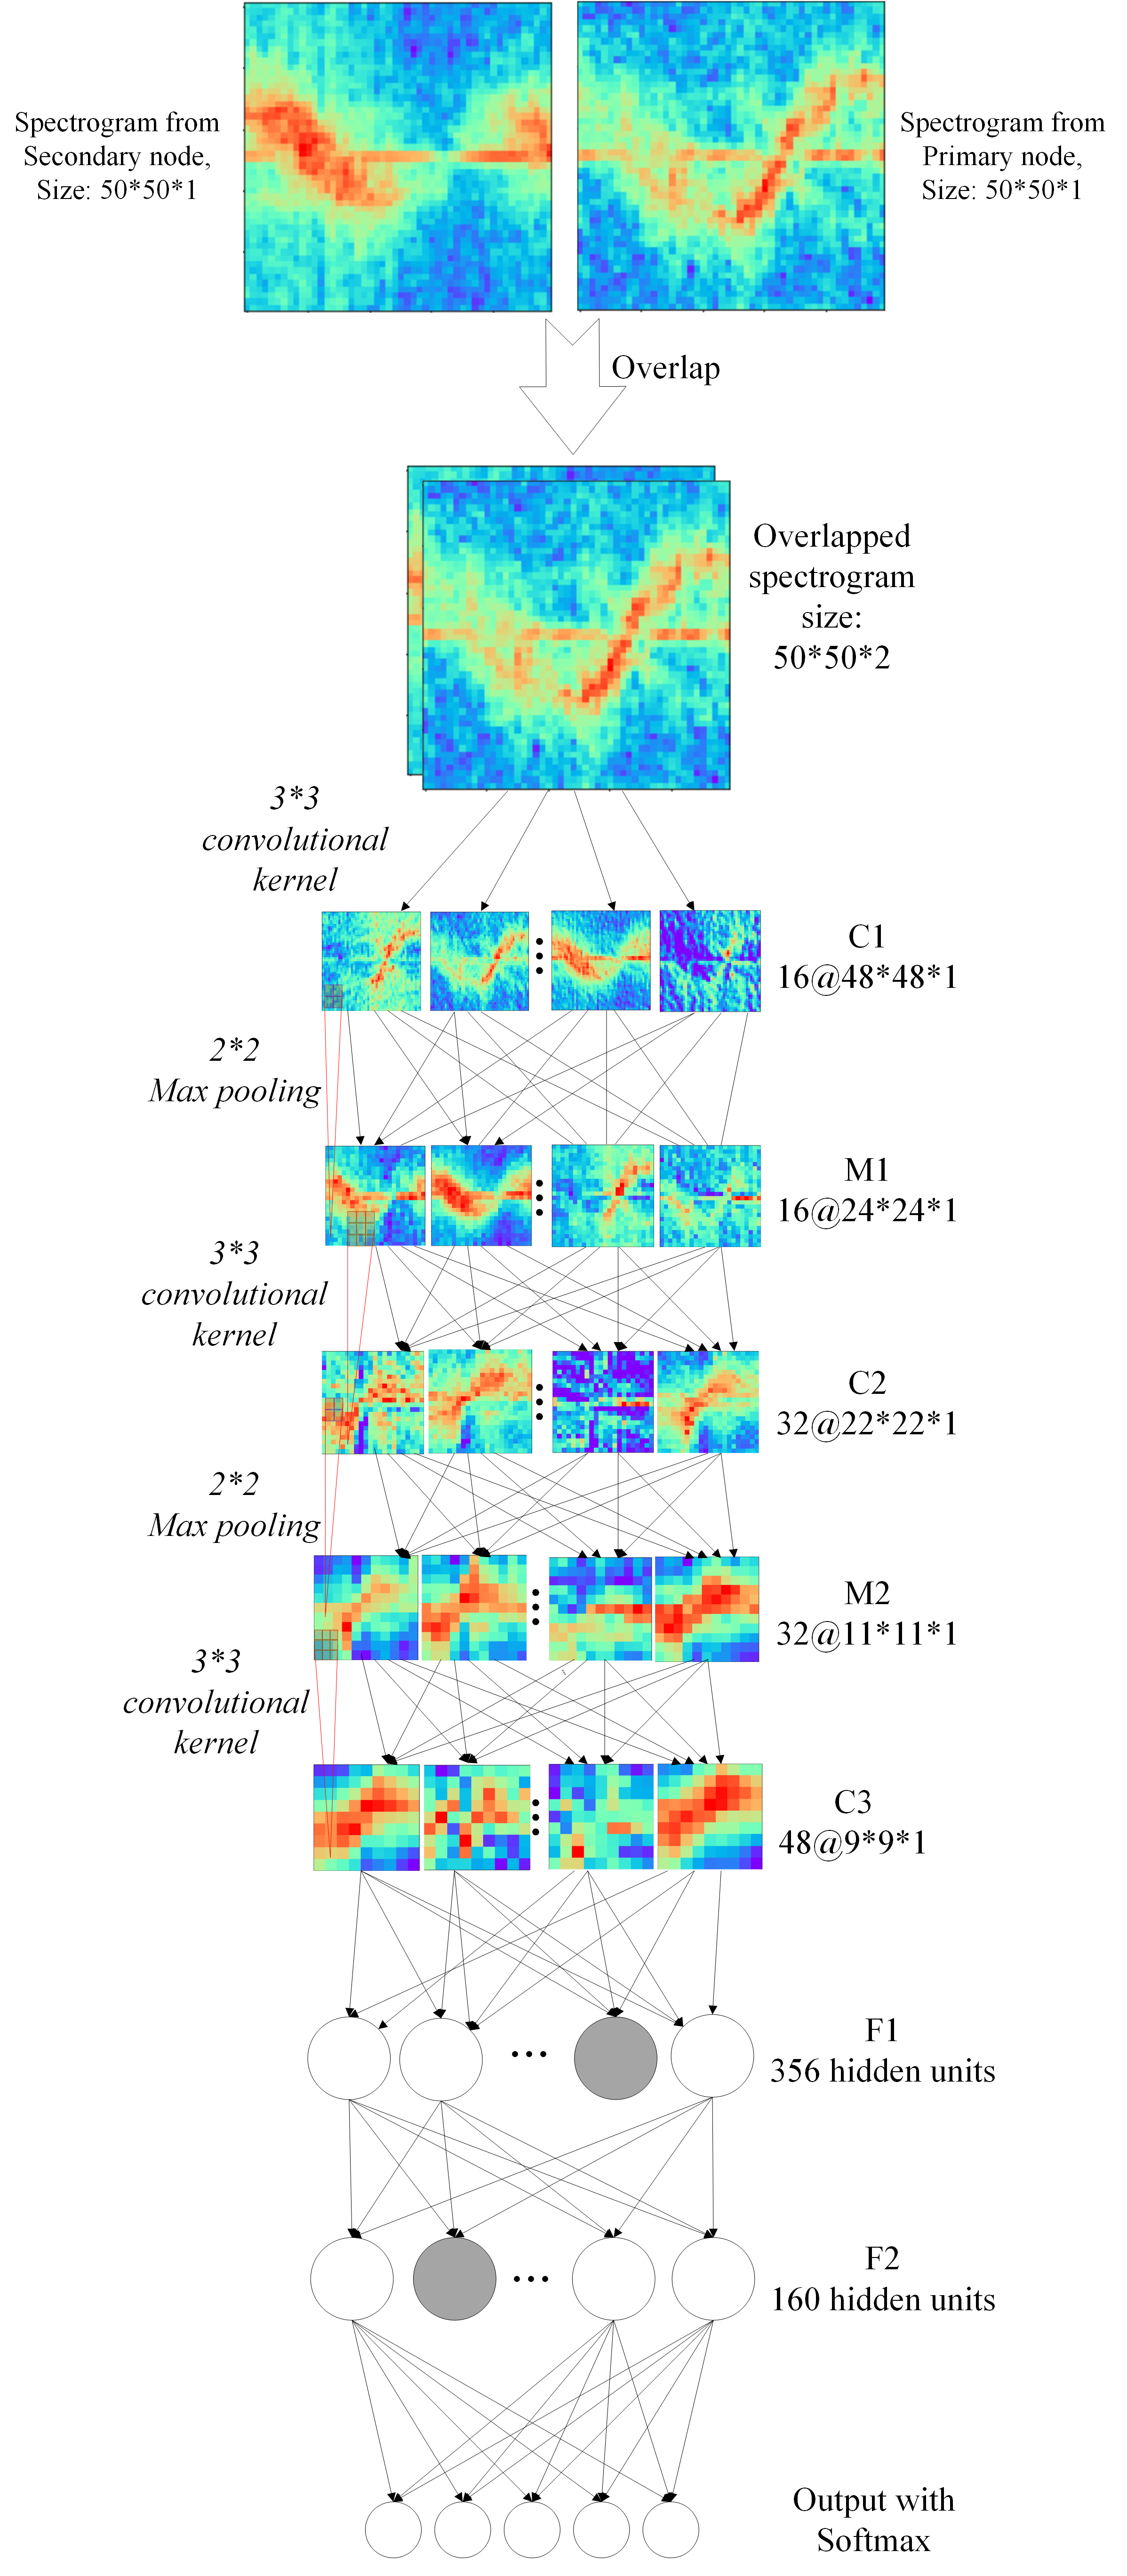
\includegraphics[width=3.6in]{cnn_}
\caption{Structure of the CNN in human behaviour detection}
\label{fig_cnn_}
\end{figure}

\subsection{Support vector machine}
As mentioned in Section I, SVM is one of the most used classifiers in micro-Doppler based human activity detection. SVMs are discrete algorithms that can be used to find the optimal separating hyperplane that maximizes the margin of the training data. A hyperplane is a decision boundary to separate data of different classes. As a dataset is usually non-linear separable in practice, the SVM algorithm is implemented using a kernel, which is a way of transforming the input data into a high-dimensional space. In the transformed feature space, it is possible to separate the data with a linear hyperplane.  An SVM with RBF (Radial basis function) kernel has been applied because a Linear SVM cannot separate the micro-Doppler data successfully.   

Differently from the works in \cite{narayanan2015radar,ccaugliyan2015micro,kim2009human,zenaldin2016radar} where the features fed into SVMs were handcrafted, the input features used in our work were extracted automatically in two ways. One way was to calculate the mean value of each column in each spectrogram and define it as a feature. Another way was applying 2D2PCA on the samples to extract the features. The results of these two feature extraction methods are compared.

Two hyperparameters $(C, gamma)$ in RBF SVM were specified manually. Cross-validation was used to tune the hyperparameters. Given a hyperparameter space  $C: [1,30],gamma:[0.1,1.0E-5]$, a different pair of parameters was selected from the hyperparameter space by the cross-validation in each training and validation iteration, in order to build a SVM classifier. The parameters that made the SVM to perform the best were considered as the optimal parameters. Table \ref{tb-svmhp} presents the optimal parameters for different classification tasks.
\begin{table}[]
\centering
\caption{Optimal hyperparameters for different classification tasks}
\label{tb-svmhp}
\begin{tabular}{|c|c|c|c|}
\hline
\textbf{Task}                                  & \textbf{Model} & \textbf{Gamma} & \textbf{C} \\ \hline
\multirow{2}{*}{Human recognition}             & SVM            & 1.0E -3.57     & 7          \\ \cline{2-4} 
                                               & SVM+2D2PCA     & 1.0E -5.84     & 3.1        \\ \hline
\multirow{2}{*}{Human activity classification} & SVM            & 1.0E -3.35     & 7.34       \\ \cline{2-4} 
                                               & SVM+2D2PCA     & 1.0E -5.67     & 5.37       \\ \hline
\multirow{2}{*}{People counting}               & SVM            & 1.0E -3.26     & 6          \\ \cline{2-4} 
                                               & SVM+2D2PCA     & 1.0E -6        & 6.5        \\ \hline
\multirow{2}{*}{Coarse-grained localization}   & SVM            & 1.0E -3.57     & 7.9        \\ \cline{2-4} 
                                               & SVM+2D2PCA     & 1.0E -6.07     & 2.9        \\ \hline
\end{tabular}
\end{table}

\subsection{\textit{k}--Nearest--Neighbor}
The \textit{k-Nearest-Neighbor} (\textit{k}NN) classification is one of the most fundamental and simple classification methods and should be one of the first choices for a classification study when there is little or no prior knowledge about the distribution of the data \cite{peterson2009k}. It also has been widely used in micro-Doppler based human activity detection\cite{ccaugliyan2015micro,erol2015kinect,gurbuz2015operational}. The \textit{k}NN classification algorithm itself is fairly straightforward and it can be summarized by the following steps: 
\begin{enumerate}
\item Choose the number for \textit{k} and a distance metric, which is commonly based on the Euclidean distance.
\item Find the \textit{k} nearest neighbors of the sample that needs to be classified
\item Assign a class label by majority vote.
\end{enumerate}

In human activity classification,  a set of features extracted from frequency spectrograms of a micro-Doppler radar can be represented by $\{f_j\}_M^N, (1 \leq j\leq M)$. Where $N$ is the number of labelled samples (frequency spectrograms),  $M$ is the number of features in each sample,  $f_j$ is the $j_{th}$ feature, and an un-labelled sample can be represented $S_i=〖\{f_j^i\} 〗_M, (1\leq j\leq M)$. In order to find $k$ closest samples to $S_i$, it is necessary to calculate the distance between each lablled sample $S_c, (1 \leq c\leq N)$ and $S_i$. A possible way to calculate this distance is using the Euclidean distance as follows:
\begin{equation}
\begin{split}
Dist(S_c,S_i)&=Dist((f_1^c,…,f_M^c ),(f_1^i,\ldots,f_M^i ))\\&=\sqrt{\sum_{p=1}^{M} (f_p^c-f_p^i)^2}
\end{split}
\end{equation}

Cross-validation is used to select a value of  \textit{k} that minimizes the overall distance between the  \textit{k} nearest labelled samples and the un-labelled sample. Finally, the unlabeled sample will be classified to the class label with a majority vote from the  \textit{k} nearest labelled samples. For each classification task, the chosen value of  \textit{k} is presented in Table \ref{tb-knn}.
% Please add the following required packages to your document preamble:
% \usepackage{multirow}
\begin{table}[]
\centering
\caption{The value \textit{k} of \textit{k}NN in different Task}
\label{tb-knn}
\begin{tabular}{|c|c|c|}
\hline
\textbf{TASK}                                  & \textbf{MODEL} & \textbf{K} \\ \hline
\multirow{2}{*}{Human recognition}             & kNN            & 1          \\ \cline{2-3} 
                                               & kNN+2D2PCA     & 1          \\ \hline
\multirow{2}{*}{Human activity classification} & KNN            & 9          \\ \cline{2-3} 
                                               & kNN+2D2PCA     & 5          \\ \hline
\multirow{2}{*}{People counting}               & KNN            & 4          \\ \cline{2-3} 
                                               & kNN+2D2PCA     & 1          \\ \hline
\multirow{2}{*}{Coarse-grained localisation}   & KNN            & 7          \\ \cline{2-3} 
                                               & kNN+2D2PCA     & 1          \\ \hline
\end{tabular}
\end{table}

\section{Result analysis}
The models built in Section VI were used to classify the samples of spectrograms. Different approaches are used to assess the accuracies obtained with these models. This section compares the performances of these models for the different classification tasks. 
\subsection{Accuracy assessment}
We compared the performances of the classifiers using different assessment methods: \begin{enumerate*} \item overall classification accuracy (OA); \item average class accuracy (AA); \item Recall; \item F1 score.\end{enumerate*} OA is given as
\begin{equation}
OA=\frac{\sum_{i=1}^{C}n_{ii}}{n}
\end{equation}
where $C$ is the number of existing classes,  $n_{ii}$ is the number of samples of class $i$ that are classified rightly in the prediction and $n$ is the total number of labeled samples used in the prediction. OA provides the rate of correctly classified samples. However, it is biased towards the classes that have a high frequency relative to other classes. Unlike OA, Recall, AA and F1 score provide an average of measures independent of class distribution. The Recall method can be calculated by
\begin{equation}
Recall=\frac{\sum_{i=1}^{C}n_{ii}}{\sum_{i=1}^{C}n_{i+}}
\end{equation}
where $n_{i+}$ represents the number of reference samples of class $i$.

The average class accuracy can be calculated by
\begin{equation}
AA=\frac{1}{C}\sum_{i=1}^{C}\frac{n_{ii}}{n_{i+}}
\end{equation}

The F1 score can be calculated by 
\begin{equation}
F1= 2 \frac{ Precision \times Recall}{Precision+Recall}
\end{equation}
where $Precision$ is given by
\begin{equation}
Precision=\frac{\sum_{i=1}^{C}n_{ii}}{\sum_{i=1}^{C}n_{+i}}
\end{equation}
where $n_{+i}$ represents the number of samples that are  predicted to be as class $i$.

Recall provides the rate of correctly classified samples of class $i, (1 \leq i\leq C)$ within all reference samples of class $i$, while AA computes the average rate of correctly classified spectrograms within each class, and F1 calculates the harmonic mean of the precision and recall.

\subsection{The Results for Human recognition}
The aim of the human recognition is to differentiate human from other targets based on their different micro-Doppler signatures. Animals are the most common confusers. In this paper, a dog was used to represent four-legged animals. According to the type of the targets, the samples were divided into four categories (e.g. human, dog, human and dog, and background/none). The performances of CNN, SVM, and \textit{k}NN are shown in Table \ref{tb-hc}. The CNN achieved the highest performance in all different metrics, with 97.5\% in OA, 96.69\% in AA, 97.23\% in Recall, and 97.22\% in F1. It outperforms SVM+2D2PCA and \textit{k}NN+2D2PCA with 1\%-7\% in OA and AA, 0.8\%-6.2\% in Recall and F1. SVM and \textit{k}NN greatly lag behind of all the others.
\begin{table}[]
\centering
\caption{Performance in human recognition}
\label{tb-hc}
\begin{tabular}{|l|l|l|l|l|}
\hline
\textbf{MODEL} & \textbf{OA} & \textbf{AA} & \textbf{RECALL} & \textbf{F1} \\ \hline
SVM            & 74.4\%      & 72.35\%     & 75.52\%         & 74.76\%     \\ \hline
SVM+2D2PCA     & 96.5\%      & 95.69\%     & 96.4\%          & 96.4\%      \\ \hline
KNN            & 66.2\%      & 64.60\%     & 66.23\%         & 65.54\%     \\ \hline
KNN+2D2PCA     & 91.1\%      & 89.69\%     & 91.41\%         & 91.24\%     \\ \hline
CNN (RadarNet) & 97.5\%      & 96.69\%     & 97.23\%         & 97.22\%     \\ \hline
\end{tabular}
\end{table}

\subsection{Results for Human activity detection}
Two types of human activities (walking and running) were investigated in the experiments. So the `human` samples can be divided into two further classes. The performances of the classifiers are shown in Table \ref{tb-had}. The best performance of 99.89\% in OA, AA, Recall, and F1 was achieved by our RadarNet, and SVM+2D2PCA follows it closely with 99.4\% in OA, 99.33\% in AA, and 99.3\% in Recall and F1. \textit{k}NN+2D2PCA also achieved a good result of 98.35\% in OA, 98.12\% in AA, 97.2\% in Recall, and 98.2\% in F1. The above three classifiers outperform SVM and \textit{k}NN by a wide margin.
\begin{table}[]
\centering
\caption{Performance in human activity detection}
\label{tb-had}
\begin{tabular}{|l|l|l|l|l|}
\hline
\textbf{MODEL} & \textbf{OA} & \textbf{AA} & \textbf{RECALL} & \textbf{F1} \\ \hline
SVM            & 86.6\%      & 87.6\%      & 85.8\%          & 88.13\%     \\ \hline
SVM+2D2PCA     & 99.4\%      & 99.33\%     & 99.3\%          & 99.38\%     \\ \hline
KNN            & 83.3\%      & 83.16\%     & 83.16\%         & 84.3\%      \\ \hline
KNN+2D2PCA     & 98.35\%     & 98.12\%     & 97.2\%          & 98.2\%      \\ \hline
CNN (RadarNet) & 99.89\%     & 99.89\%     & 99.89\%         & 99.89\%       \\ \hline
\end{tabular}
\end{table}

\subsection{Results for People counting}
In \textit{Case 1}, the micro-Doppler signatures of a single person were collected. In \textit{Case 2}, samples for groups of two, three, and four people were collected by our radar system. So for people counting, the `human`' samples can be further divided into four classes according to the number of people. The performances of the classifiers in people counting are shown in Table \ref{tb-pc}. RadarNet still achieved the best performance results with 98.85\% in OA, 98\% in AA, 98.85\% in Recall, and 98.7\% in F1, followed by SVM+2D2PCA with 95.9\% in OA, 95.7\% in AA, and 95.9\% in Recall and F1. The performance of \textit{k}NN+2D2PCA lags behind SVM+2D2PCA with around 12.5\% in OA, AA, Recall, and F1. SVM and \textit{k}NN had very poor performances in people counting.
\begin{table}[]
\centering
\caption{Performance in people counting}
\label{tb-pc}
\begin{tabular}{|l|l|l|l|l|}
\hline
\textbf{MODEL} & \textbf{OA} & \textbf{AA} & \textbf{RECALL} & \textbf{F1} \\ \hline
SVM            & 65.3\%      & 58\%        & 65.3\%          & 63\%        \\ \hline
SVM+2D2PCA     & 95.9\%      & 95.7\%      & 95.9\%          & 95.9\%      \\ \hline
KNN            & 60.46\%     & 52.6\%      & 61\%            & 58.4\%      \\ \hline
KNN+2D2PCA     & 83.3\%      & 83.4\%      & 81.88\%         & 83.4\%      \\ \hline
CNN (RadarNet) & 98.85\%     & 98\%        & 98.85\%         & 98.7\%      \\ \hline
\end{tabular}
\end{table}

\subsection{Results for Coarse-grained localization of human targets}
In the experiments, the detection area was split into three non-overlapping ranges, which were 1-3m, 3-5m, and 5-7m relative to the primary node. The coarse-grained localization estimates which range the location of the human target belongs to. With these three ranges, the samples of the human target were divided into three categories. The performances of the classifiers for coarse-grained localization are shown in Table \ref{tb-loc}. The overall performance achieved in coarse-localization is higher than other three classification tasks. The CNN perfectly estimated the range where the target was located in. SVM+2D2PCA presented slight inferior results, with 99.9\% in OA, and 99.87\% in AA, Recall, and F1. \textit{k}NN+2D2PCA also performed very well with the lowest accuracy metric achieving 99.19\%. SVM underperformed SVM+2D2PCA by around 12\% in the different accuracy metrics, with around 88\% in OA, Recall and F1, and 87.25\% in AA. Finally, \textit{k}NN presented the lowest scores, achieving a percentage of around 81\% in the different metrics.
\begin{table}[]
\centering
\caption{Performance in Coarse-grained localization}
\label{tb-loc}
\begin{tabular}{|l|l|l|l|l|}
\hline
\textbf{MODEL} & \textbf{OA} & \textbf{AA} & \textbf{RECALL} & \textbf{F1} \\ \hline
SVM            & 88.2\%      & 87.25\%     & 88\%            & 88\%        \\ \hline
SVM+2D2PCA     & 99.9\%      & 99.87\%     & 99.87\%         & 99.87\%     \\ \hline
KNN            & 81.8\%      & 81.42\%     & 81.08\%         & 81\%        \\ \hline
KNN+2D2PCA     & 99.19\%     & 99.24\%     & 99.19\%         & 99.19\%     \\ \hline
CNN (RadarNet) & 100\%       & 100\%       & 100\%           & 100\%       \\ \hline
\end{tabular}
\end{table}

\subsection{Analysis}
Based on the above results achieved by the classifiers in four different classification tasks, the chart presented in Fig. \ref{fig_rsu} was plotted. It is clear from the chart that, in all four tasks, the highest performance (OA) of the classifiers is given by the CNN (RadarNet), followed by the SVM+2D2PCA, then \textit{k}NN+2D2PCA. The classifiers with lower accuracy results were SVM and \textit{k}NN. As one of the most popular deep learning algorithms, CNN proved to be very suitable for micro-Doppler signature-based classification. CNN achieved the best OA scores, which were 97.5\% in human recognition, 99.89\% in human activity detection, 98.85\% in people counting, and 100\% in coarse-grained localization. SVM+2D2PCA follows closely and \textit{k}NN+2D2PCA is slightly inferior to SVM+2D2PCA, but both of them exceeded SVM and \textit{k}NN by a wide margin between 11\%-18\%. The performances of SVM and \textit{k}NN were greatly improved by the features extraction using 2D2PCA.   

From the aspect of classification tasks, different classification tasks have different levels of difficulty, which indicates whether samples in a classification task are easier or more difficult to be classified. If the tasks are sorted by order of difficulty, the order would be: $People\;  Counting> Human\;  Recognition>Human\;  Activity\;  Detection>Rough\;  localization$. This can be seen in Fig. \ref{fig_rsu}, the average performance of all classifiers for coarse-grained localization is the highest compared to the average performance of the other classification tasks, followed by the average for human detection and human recognition. While the average accuracy results for people counting are the lowest of all. Fig. \ref{fig_confusion} shows the \textit{confusion matrices} of CNNs for the four classification tasks. A \textit{confusion maxtrix} is a table used to describe the performance of a classification model (or `‘classifier`’) on a set of test data for which the true values are known. All correct predictions are located in the diagonal of the table. It allows the visualization of the performance of a classifier. In Fig. \ref{fig_confusion}(a), the most misclassified samples were from the `‘Human and Dog`’, and they were classified into `‘Human`’. This implies that it is relatively difficult to differentiate the micro-Doppler signatures of these two classes. In Fig. \ref{fig_confusion}(b), six samples of `‘Walking`’ were classified into `‘Running`’, this could be probably because different participants have different walking speeds, and fast-walking people and slow-running people generated more similar micro-Doppler signatures that is harder to differentiate. Fig. \ref{fig_confusion}(c) presents 12 out 13 misclassified samples of `‘1 person`’ that were classified into `‘2 people`’; 13 out of 14 samples of `‘2 people`’ were misclassified as  `‘1 person`’, and 17 samples of `‘3 people`’ were misclassified as `‘4 people`’. This indicates that adjacent categories are more likely to be misclassified between each other for the case of people counting. This is because there are more similarities in the micro-Doppler signatures between adjacent categories of people counting.

\subsection{Comparison with the related work}
There are some other similar works that is worth to compare with our study. In human and animal classification, the authors of \cite{lee2017classification} used a two-layer CNN to classify two different categories of targets: dog and human. Each sample was collected independently in an environment with low-level of clutter using similar BumbleBee radars. They achieved an OA of 100\%. Differently, our samples were collected continuously in wild outdoor areas and they reflect better the naturally continuous human movement in a realistic environment with high-levels of clutter (for example, foliage and branch tree movement with wind). We considered four categories of targets (human, dog, human and dog, and background), therefore the complexity of the target classification was higher. If we only consider the same two categories as \cite{lee2017classification} (e.g. dog and human) our classification also achieves 100\% overall accuracy as shown in Fig. \ref{fig_confusion} (a). 

The authors in \cite{miller2013micro} also investigated confusers, they aimed to differentiate the categories of human walking and horse walking in an outdoor scenario. They used a Doppler radar operating at 9.2 GHz, which works in a higher frequency than the Bumblebee radar, but it consumes more energy. They achieved an OA of 92.7\% in classification between humans and horses using SVM. Although our confuser was a different animal, we achieved a better result. This indicates that the performance of the human detection using micro-Doppler signatures depends on both the classifier and the radars. Although the radar used in \cite{miller2013micro} has better frequency and distance resolutions than the Bumblebee radar, a well modeled CNN is able to compensate these limitations.

In human activity classification, the authors in \cite{zenaldin2016radar} investigated three motions (crawling, walking, and jogging) in four different environments, including (a) free space, (b) through-the-wall, (c) leaf tree foliage, and (4) needle tree foliage. They made their experiments using a continuous-wave Doppler radar operating at 6.5 GHz. They implemented an SVM classifier. The best classification results were obtained from the experiments in free space, where it was achieved an overall accuracy of above 91\%, followed by the experiments in leaf tree foliage and in through-the-wall. The lowest classification rate was from the experiments in needle tree foliage of around 71\% OA. In our work, we only considered the classification of two activities (walking and running), but we could argue that we performed the experiments in an environment comparable to the leaf tree foliage and the needle tree foliage with considerably better results.  In \cite{zenaldin2016radar}, the authors used the BumbleBee radar to measure micro-Doppler signatures of three motions (walking, running, and crawling) in an indoor scenario. The classification was implemented using the \textit{k}NN method. Their classifier correctly classified the activity of walking 90\% of the cases, 88\% for running, and 93\% for crawling. Although the radar used in \cite{zenaldin2016radar} is the same as ours, they made the experiments in less noisy conditions (indoor environment), but their results are still not comparable to the 99.8\% OA that we achieved in our work.

For people counting, the authors in \cite{tahmoush2009radar} applied a Ka-band Doppler radar to measure the micro-Doppler signatures of people in outdoors. The stride rate over the peak period was extracted from spectrograms as an important feature to classify whether the target was an individual or a small group. With a nearest neighbor classification approach, they achieved over 80\% classification rate in overall. The authors in \cite{trommel2016multi} measured the simulated walking of subjects using a simulated CW radar. They varied the subjects from no subject to a group of five people. The classifications were performed using a DCNN on the simulated data and achieved a high accuracy of 96.1\% in overall. However, real environments are far more complex than simulations, therefore our 98.85\% overall accuracy in people counting is a good performance result.

For coarse-grained localization using micro-Doppler, to the best of our knowledge, there is still no relevant and comparable work. 

Although the comparison we make cannot be directly applied to the cited related work above, it is plausible to infer that the methods, including the signal processing and the classifiers, used in this research are solid implementation tools to be used with micro-Doppler signatures in order to perform human activity detection in outdoors. The comparative performance is even better for human activity classification and people counting.
\begin{figure}[!t]
\centering
%\captionsetup{justification=centering}
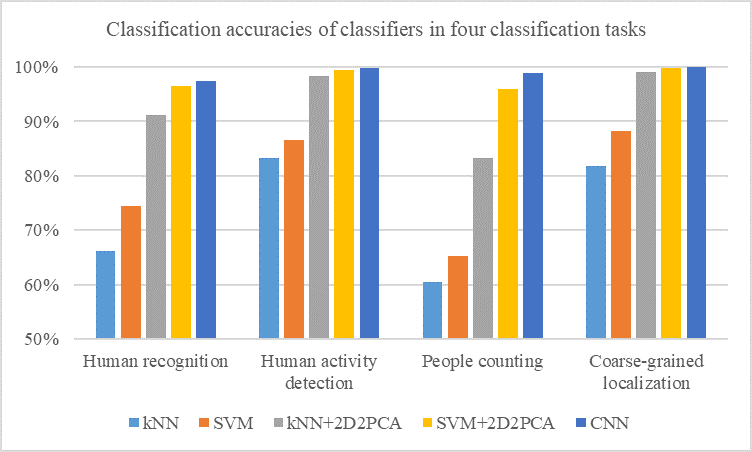
\includegraphics[width=3.6in]{result}
\caption{The performances of five classifiers in four classification tasks}
\label{fig_rsu}
\end{figure}

\begin{figure}[!t]
\centering
%\captionsetup{justification=centering}
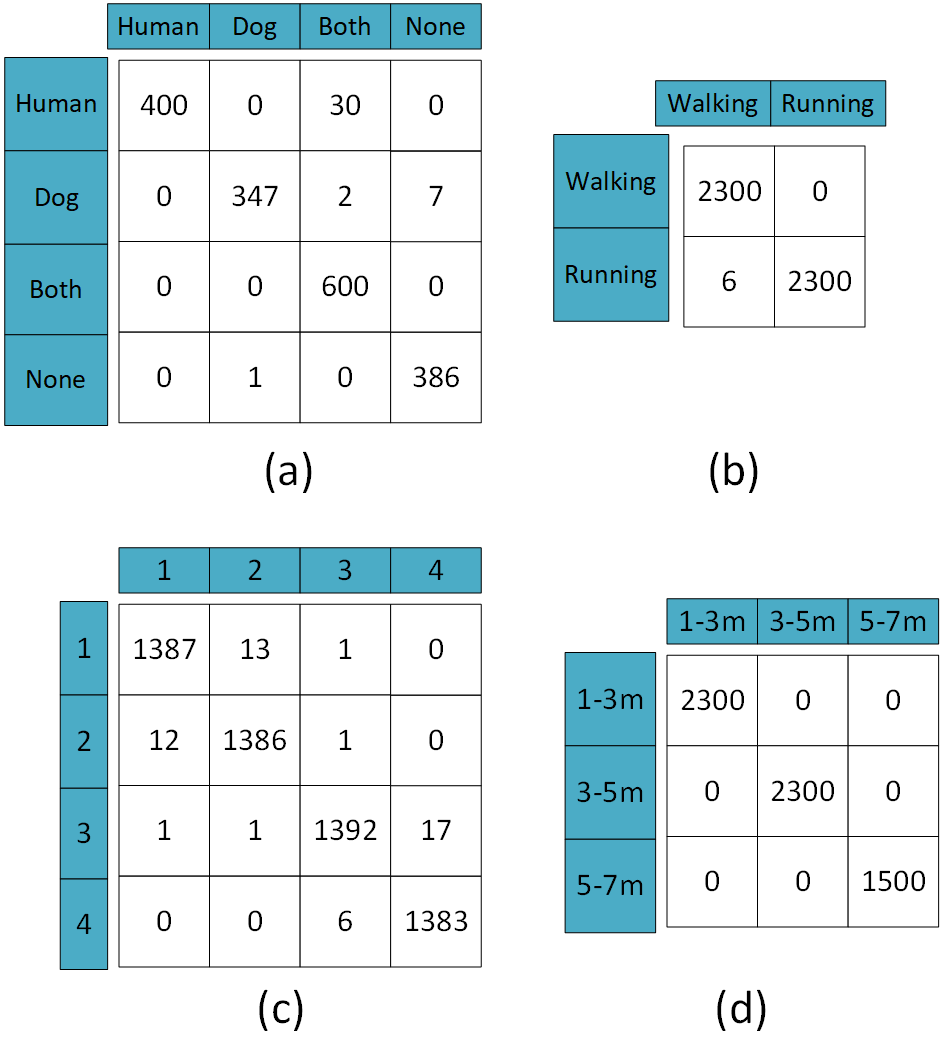
\includegraphics[width=3.4in]{confusion}
\caption{Confusion matrices of CNNs in (a). Human recognition, (b). Activity detection, (c). People counting, (d). Coarse-grained localization}
\label{fig_confusion}
\end{figure}



\section{Factors in micro-Doppler based classification}
In this section, three factors, including the frame length of the sliding window, the angle of the movement, and the number of radars are investigated in micro-Doppler based classification. It is helpful to assess the influence of these factors on micro-Doppler data processing and model optimization, and make the micro-Doppler based human activity analysis more practical.
\begin{figure*}[!ht]
         \centering
         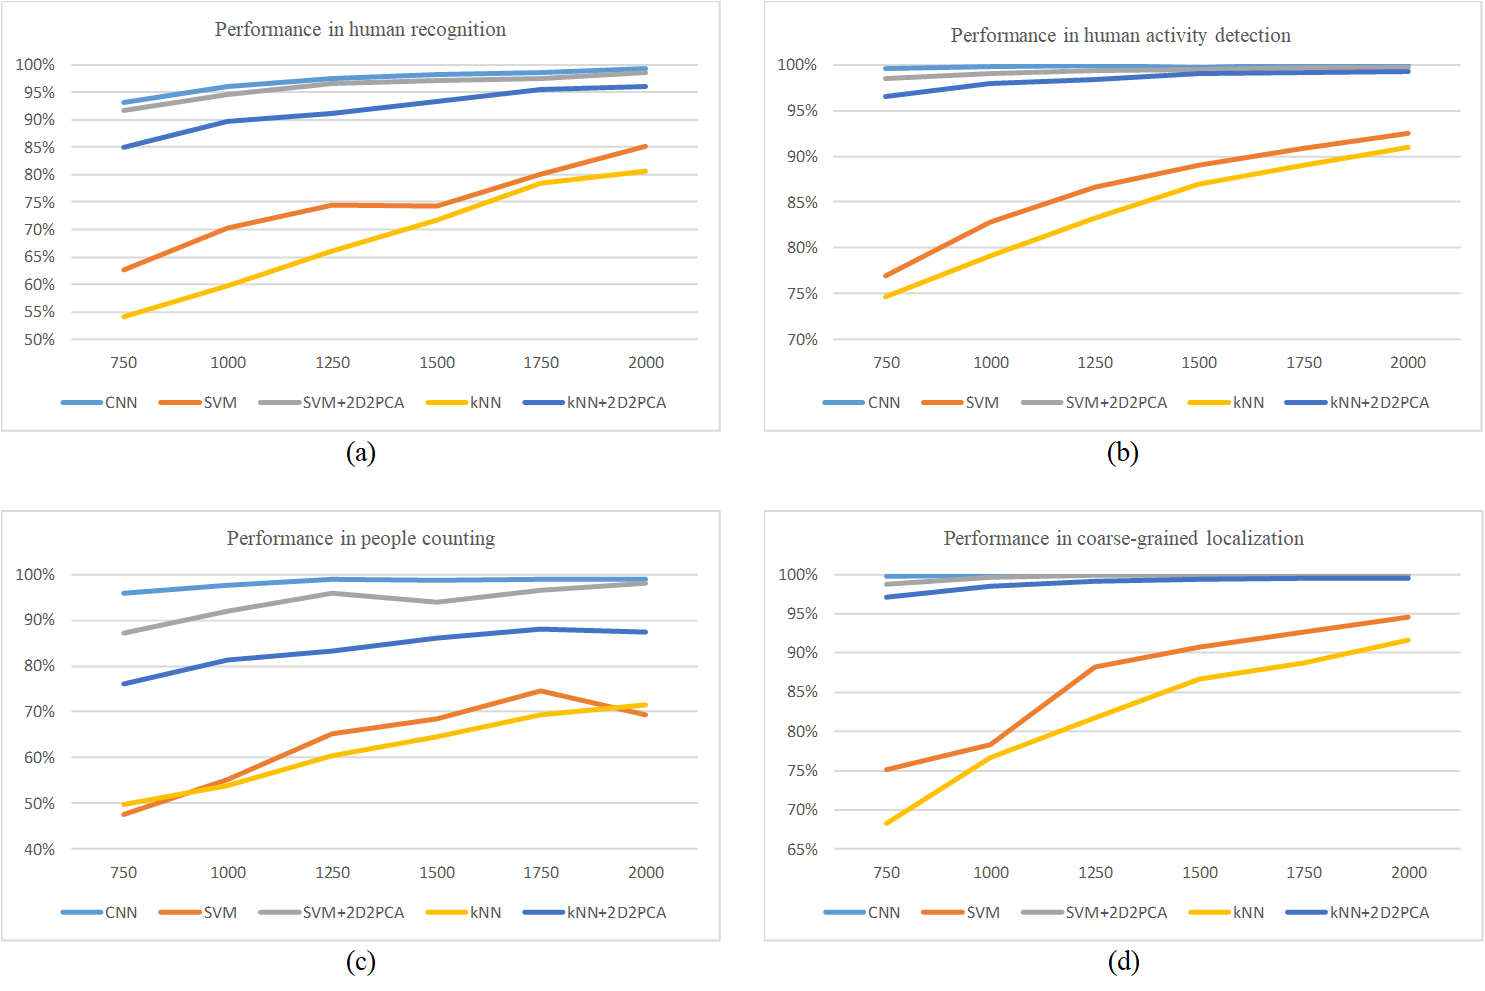
\includegraphics[width=6.8in]{frames}
         \caption{Performances (OA) of the classifiers with the changing frame lengths}
         \label{fig_frames}
\end{figure*}
\subsection{The frame length of the sliding window}
As mentioned in Section IV, the radar signals are processed with STFT, which uses a sliding window with a given frame length to generate spectrograms. It is worth studying how the different frame lengths affect the classification. 

Six frame lengths, including 750 samples, 1000 samples, 1250 samples, 1500 samples, 1750 samples, and 2000 samples are investigated here. As the sample frequency is 250 Hz, the frame length also can be measured in the time domain. Then the six frame lengths also can be measured as 3s, 4s, 5s, 6s, 7s, and 8s. With the generated samples, the classifiers are used to perform the classification. As shown in Fig. \ref{fig_frames}, the performances (OA used) of almost all classifiers increase with the increasing frame length for all four classification tasks. Although the amount of the increase declines for greater frame lengths. The superiority of the classifier’s performance remains the same as stated in section VII, which is still $CNN>(SVM+2D2PCA)>(kNN+2D2PCA)>SVM>kNN$. Therefore, it is plausible to conclude that increasing the frame length of the sliding window can increase the classification accuracy. A longer frame length means the sliding window contains more information that makes the classification easier. In reality, it is not possible to increase the frame length endlessly, because each activity has a time period. Also, a longer frame length means a longer sampling time interval that results in higher latency, which delays the classification results. So, the frame length is determined based on the tradeoff between the classification accuracy and the latency. The frame length used in this research was 5s, which led to good accuracies and low latency. Also, the time of 5s was a suitable period to measure the movement in detection area, because the walking or the running along the detection area usually took 4-7s.

\subsection{Angles of the movement}
In Section III, we stated that the experiments were made from three different angles ($\ang{0}$, $\ang{45}$, and $\ang{90}$). The coarse-grained localization made in \textit{Case 3} was investigated from two angles ($\ang{45}$ and $\ang{90}$). As shown in Fig. \ref{fig_angles}, the classifications for human activity detection and people counting performed best with samples from $\ang{0}$ that reached 100\% and 99.46\% overall accuracies for the respective classification tasks. Samples from \ang{45} produced the worst results, which were 99.7\% and 97.7\% in human activity detection and people counting respectively. For the coarse-grained localization, the same OA (100\%) was achieved at both \ang{45} and \ang{90}. It means the angle of the movements has little effect to the classification accuracy in localization. In conclusion, the direction of the movement to the radar beam can affect the classification in human activity and people counting, and \ang{0} can provide the best accuracy, followed by \ang{90} and \ang{45}. This is probably because the RCS is largest when people move at \ang{0}.  While for the coarse-grained localization, the angle of movement direction had no practical effect.
\begin{figure}[!ht]
         \centering
         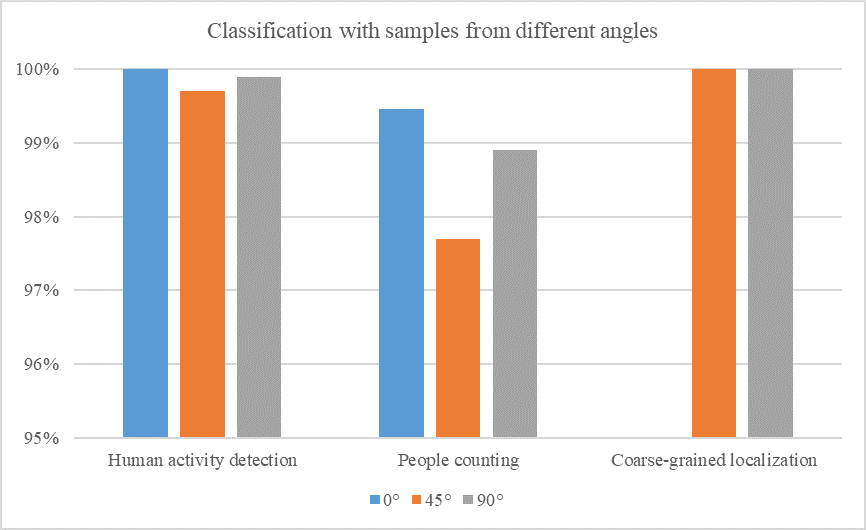
\includegraphics[width=3.5in]{angles}
         \caption{Performances of the classifiers in the tasks with the changing frame lengths}
         \label{fig_angles}
\end{figure}
\subsection{Number of Doppler Radars}
The radar system built in this research consisted of two radars. In the data processing, the signals from both radars were fused together. In this section, we investigate how the number of radars affects the classification results. For this purpose, a new CNN model 'RadarNet\textsubscript{new}' was trained using only the data from the primary radar node. 
\begin{table}[]
\centering
\caption{Structure of RadarNet and RadarNet\textsubscript{new}}
\label{tb-srr}
\begin{tabular}{|c|c|}
\hline
\textbf{RadarNet} & \textbf{RadarNet\textsubscript{new}} \\ \hline
X ($50\times 50\times 2$)       & X ($50\times50\times1$)          \\ \hline
Conv1-16@$48\times48\times1$  & Conv1-12@$48\times48\times1$     \\ \hline
maxpool           & Maxpool              \\ \hline
BN                & BN                   \\ \hline
Conv2-32@$22\times22\times1$  & Conv2-24@$22\times22\times1$     \\ \hline
maxpool           & Maxpool              \\ \hline
BN                & BN                   \\ \hline
Dropout (0.3)     & Dropout (0.3)        \\ \hline
Conv3-48@$9\times9\times1$    & Conv3-24@$9\times9\times1$       \\ \hline
Flatten           & Flatten              \\ \hline
BN                & BN                   \\ \hline
Dropout (0.4)     & Dropout (0.4)        \\ \hline
FCL-350           & FCL-256              \\ \hline
BN                & BN                   \\ \hline
Dropout (0.3)     & Dropout (0.3)        \\ \hline
FCL-160           & FCL-76               \\ \hline
\multicolumn{2}{|c|}{FCL (Softmax)}      \\ \hline
\end{tabular}
\end{table}

The main difference between RadarNet\textsubscript{new} and RadarNet is the input size, which is $50\times 50\times 1$ for RadarNet\textsubscript{new}, and $50\times 50\times 2$ for RadarNet. Because one radar generates one spectrogram at each time step, the shape of each spectrogram is $50\times 50\times 1$. As seen in Table \ref{tb-srr}, the structure of both CNNs are very similar, both contain 3 convolutional layers, 2 max-pooling layers, and 2 fully connected layers. However, RadarNet\textsubscript{new} presents less feature maps and hidden units. The comparison of their performances is shown in Fig. \ref{fig_radars}. As it can be noted, the performance obtained from two radars is higher than the performance obtained by using only one radar in all four classification tasks. For human activity detection and coarse-grained localization, the results presented by the CNN using data from one radar were slightly inferior to those of using data from two radars. While in human recognition, and especially in people counting, the overall accuracy scores obtained by the data from two radars exceeded those from one radar by a large margin. In people counting, the overall accuracy score with one radar data was 91.57\%, while for two radar data it reached 98.85\%. In human recognition, the overall accuracy with one radar was 95.70\%, while the one with two radars reached 97.5\%. It is plausible to conclude that increasing the number of radars the accuracy of micro-Doppler based classification also increases. However, this increase is very small to human activity detection and coarse-grained localization, but very obvious to human recognition and people counting.
\begin{figure}[!ht]
         \centering
         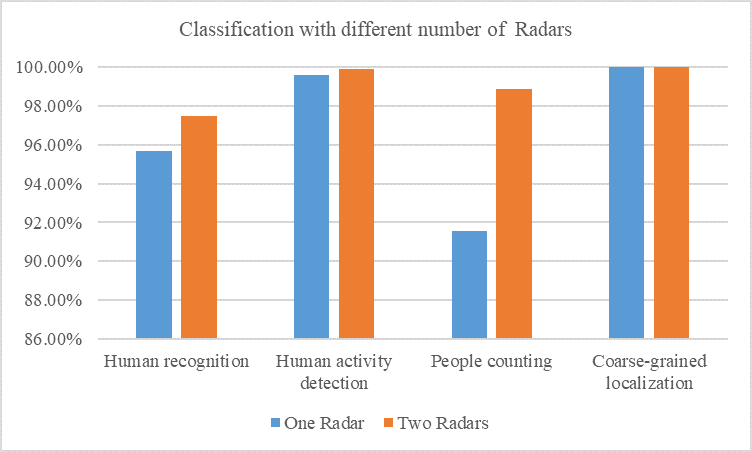
\includegraphics[width=3.5in]{radars}
         \caption{CNN classification with samples of different number of radars}
         \label{fig_radars}
\end{figure}

\section{Conclusion}
This paper applied micro-Doppler signatures to perform four classification tasks, which are human recognition, human activity classification, people counting, and coarse-grained localization. A radar system that consists of two pulsed Doppler radars operating at 5.8 GHz was built. With the collected radar signals and processing them with STFT, the patterns of the spectrograms of different subjects, activities, location ranges, and the number of people were presented and analyzed. Five classifiers, including CNN (RadarNet), SVM, SVM+2D2PCA, \textit{k}NN, \textit{k}NN+2D2PCA were implemented. It was found that the CNN performs the best in all four classification tasks. Also, 2D2PCA was proved to be a very good feature extraction method in micro-Doppler analysis and improved the performance of SVM and \textit{k}NN significantly. At last, three factors, including the frame length of the sliding window, the angle of the movement, and the number of radars were investigated for micro-Doppler signature applications. Our investigation provided a valuable guideline for model optimization and experiment setup of micro-Doppler based research and applications.

In conclusion, this research validates low-power low-cost radars have a great potential for human activity detection, even in outdoor environments with high-levels of clutter. In future work, the method used in this research will be extrapolated into a Doppler radar with a greater detection range and extended to more application scenarios.


% needed in second column of first page if using \IEEEpubid
%\IEEEpubidadjcol


% An example of a floating figure using the graphicx package.
% Note that \label must occur AFTER (or within) \caption.
% For figures, \caption should occur after the \includegraphics.
% Note that IEEEtran v1.7 and later has special internal code that
% is designed to preserve the operation of \label within \caption
% even when the captionsoff option is in effect. However, because
% of issues like this, it may be the safest practice to put all your
% \label just after \caption rather than within \caption{}.
%
% Reminder: the "draftcls" or "draftclsnofoot", not "draft", class
% option should be used if it is desired that the figures are to be
% displayed while in draft mode.
%
%\begin{figure}[!t]
%\centering
%\includegraphics[width=2.5in]{myfigure}
% where an .eps filename suffix will be assumed under latex, 
% and a .pdf suffix will be assumed for pdflatex; or what has been declared
% via \DeclareGraphicsExtensions.
%\caption{Simulation results for the network.}
%\label{fig_sim}
%\end{figure}

% Note that the IEEE typically puts floats only at the top, even when this
% results in a large percentage of a column being occupied by floats.


% An example of a double column floating figure using two subfigures.
% (The subfig.sty package must be loaded for this to work.)
% The subfigure \label commands are set within each subfloat command,
% and the \label for the overall figure must come after \caption.
% \hfil is used as a separator to get equal spacing.
% Watch out that the combined width of all the subfigures on a 
% line do not exceed the text width or a line break will occur.
%
%\begin{figure*}[!t]
%\centering
%\subfloat[Case I]{\includegraphics[width=2.5in]{box}%
%\label{fig_first_case}}
%\hfil
%\subfloat[Case II]{\includegraphics[width=2.5in]{box}%
%\label{fig_second_case}}
%\caption{Simulation results for the network.}
%\label{fig_sim}
%\end{figure*}
%
% Note that often IEEE papers with subfigures do not employ subfigure
% captions (using the optional argument to \subfloat[]), but instead will
% reference/describe all of them (a), (b), etc., within the main caption.
% Be aware that for subfig.sty to generate the (a), (b), etc., subfigure
% labels, the optional argument to \subfloat must be present. If a
% subcaption is not desired, just leave its contents blank,
% e.g., \subfloat[].


% An example of a floating table. Note that, for IEEE style tables, the
% \caption command should come BEFORE the table and, given that table
% captions serve much like titles, are usually capitalized except for words
% such as a, an, and, as, at, but, by, for, in, nor, of, on, or, the, to
% and up, which are usually not capitalized unless they are the first or
% last word of the caption. Table text will default to \footnotesize as
% the IEEE normally uses this smaller font for tables.
% The \label must come after \caption as always.
%
%\begin{table}[!t]
%% increase table row spacing, adjust to taste
%\renewcommand{\arraystretch}{1.3}
% if using array.sty, it might be a good idea to tweak the value of
% \extrarowheight as needed to properly center the text within the cells
%\caption{An Example of a Table}
%\label{table_example}
%\centering
%% Some packages, such as MDW tools, offer better commands for making tables
%% than the plain LaTeX2e tabular which is used here.
%\begin{tabular}{|c||c|}
%\hline
%One & Two\\
%\hline
%Three & Four\\
%\hline
%\end{tabular}
%\end{table}


% Note that the IEEE does not put floats in the very first column
% - or typically anywhere on the first page for that matter. Also,
% in-text middle ("here") positioning is typically not used, but it
% is allowed and encouraged for Computer Society conferences (but
% not Computer Society journals). Most IEEE journals/conferences use
% top floats exclusively. 
% Note that, LaTeX2e, unlike IEEE journals/conferences, places
% footnotes above bottom floats. This can be corrected via the
% \fnbelowfloat command of the stfloats package.





% if have a single appendix:
%\appendix[Proof of the Zonklar Equations]
% or
%\appendix  % for no appendix heading
% do not use \section anymore after \appendix, only \section*
% is possibly needed

% use appendices with more than one appendix
% then use \section to start each appendix
% you must declare a \section before using any
% \subsection or using \label (\appendices by itself
% starts a section numbered zero.)
%



% use section* for acknowledgment
\section*{Acknowledgment}


This research was funded in part by a China Scholarship Council (CSC) and QMUL PhD Grant. The authors would also like to thank Mahadi Hasan for assisting the first set up of the radar devices and to all participants who joined the experiments.


% Can use something like this to put references on a page
% by themselves when using endfloat and the captionsoff option.
\ifCLASSOPTIONcaptionsoff
  \newpage
\fi



% trigger a \newpage just before the given reference
% number - used to balance the columns on the last page
% adjust value as needed - may need to be readjusted if
% the document is modified later
%\IEEEtriggeratref{8}
% The "triggered" command can be changed if desired:
%\IEEEtriggercmd{\enlargethispage{-5in}}

% references section

% can use a bibliography generated by BibTeX as a .bbl file
% BibTeX documentation can be easily obtained at:
% http://mirror.ctan.org/biblio/bibtex/contrib/doc/
% The IEEEtran BibTeX style support page is at:
% http://www.michaelshell.org/tex/ieeetran/bibtex/
%\bibliographystyle{IEEEtran}
% argument is your BibTeX string definitions and bibliography database(s)
%\bibliography{IEEEabrv,../bib/paper}
%
% <OR> manually copy in the resultant .bbl file
% set second argument of \begin to the number of references
% (used to reserve space for the reference number labels box)
% \begin{thebibliography}{1}

% \bibitem{IEEEhowto:kopka}
% H.~Kopka and P.~W. Daly, \emph{A Guide to \LaTeX}, 3rd~ed.\hskip 1em plus
%   0.5em minus 0.4em\relax Harlow, England: Addison-Wesley, 1999.

% \end{thebibliography}

% biography section
% 
% If you have an EPS/PDF photo (graphicx package needed) extra braces are
% needed around the contents of the optional argument to biography to prevent
% the LaTeX parser from getting confused when it sees the complicated
% \includegraphics command within an optional argument. (You could create
% your own custom macro containing the \includegraphics command to make things
% simpler here.)
%\begin{IEEEbiography}[{\includegraphics[width=1in,height=1.25in,clip,keepaspectratio]{mshell}}]{Michael Shell}
% or if you just want to reserve a space for a photo:

\bibliographystyle{IEEEtran}
\bibliography{bibtex/bib/Biblio}

\begin{IEEEbiography}[{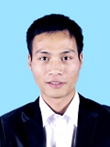
\includegraphics[width=1in,height=1.25in,clip,keepaspectratio]{fei}}]{Fei Luo}
received the B.Sc. degree in Geographic Information System for Jiangxi University of Science and Technology, Jiangxi, China, in 2008, and the M.sc. degree in Surveying and Mapping from Wuhan University, Wuhan, China, in 2016. He is currently pursuing the Ph.D. degree in Electronic Engineering in the School of Electronic Engineering and Computer Science. His research interests include Geographic information system, human activity detection, Machine learning.
\end{IEEEbiography}


% insert where needed to balance the two columns on the last page with
% biographies
%\newpage

\begin{IEEEbiography}[{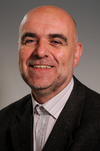
\includegraphics[width=1in,height=1.25in,clip,keepaspectratio]{stefan}}]{Stefan Poslad}
received the B.Sc. degree in physics from the University of Southampton, Southampton, U.K., the M.Sc. degree in medical physics from the University of Aberdeen, Aberdeen, U.K., and the Ph.D. degree from Newcastle University, Newcastle upon Tyne, U.K., in 1987, focusing on artificial lung sensing during open heart surgery. Since 2000, he has been a Principal Investigator of 12 funded collaborative research projects, and has received funding from the U.K. Research Council, Europe, Norway, the U.S., and from the industry.
\end{IEEEbiography}

% if you will not have a photo at all:
\begin{IEEEbiography}[{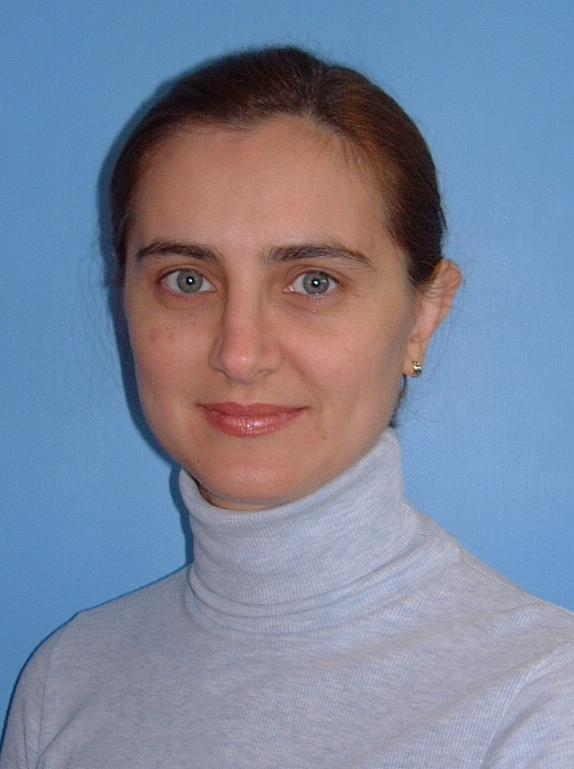
\includegraphics[width=1in,height=1.25in,clip,keepaspectratio]{eliane}}]{Elaine Bodanese}
MSc, Ph.D., MIEEE, joined Queen Mary University of London in 2003. She is a senior lecturer in the School of Electronic Engineering and Computer Science and a member of the Networks Research Group. Dr Bodanese received her Electrical Engineering degree from the Federal University of Parana (Brazil) and her M.Sc. degree in Electrical Engineering from the Federal University of Santa Catarina (Brazil). In 2000, she received her Ph.D. in Electronic Engineering from Queen Mary, University of London (UK). Her research interests include next generation wireless systems, dynamic radio resource management for heterogeneous wireless environments, communication support for emergencies, cooperative communications, ad hoc and sensor networks, the Internet of Things, and wireless localization.
\end{IEEEbiography}

% You can push biographies down or up by placing
% a \vfill before or after them. The appropriate
% use of \vfill depends on what kind of text is
% on the last page and whether or not the columns
% are being equalized.

%\vfill

% Can be used to pull up biographies so that the bottom of the last one
% is flush with the other column.
\enlargethispage{0in}


% that's all folks
\end{document}


